% This is the main TeX document for the guide for teaching assistants in
% dynamics at AM:BM.
%
% Note that this file as well as the title page are derived from documents
% handed out by Samir Omerovic of the Institute of Structural Analysis of
% TU Graz.  
%
% This project is version-controlled by git.
%
%%%%%%%%%%%%%%%%%%%%%%%%%%%%%%%%%%%%%%%%%%%%%%%%%%%%%%%%%%%%%%%%%%%%%%%%%%%%%%%%
\documentclass[
a4paper,            % defines the paper size: a4paper (default), a5paper
BCOR20mm,           % Bindekorrektur
twoside,            % changes to a two-page-layout (alternatively: oneside)
parskip=half,       % insert an empty line between two paragraphs (skip, ...)
openright,          % open chapter on right hand side
]{scrreprt}

%%%%%%%%%%%%%%%%%%%%%%%%%%%%%%%%%%%%%%%%%%%%%%%%%%%%%%%%%%%%%%%%%%%%%%%%%%%%%%%%
%%% PACKAGES
\usepackage{amsmath,amssymb,amstext,wasysym}
\usepackage{blkarray}
\usepackage[ngerman]{babel}             % ngerman: language set to new-german
\usepackage[utf8]{inputenc}             % coding of german special characters
                                        % (in windows perhaps 'ansinew' has to
                                        %  be used instead of 'utf8')
\usepackage{ae,aecompl}                 % ae, aecompl: coding of characters in
                                        % PDF documents
\usepackage{listings}                   % listings: include programming code
\usepackage{units}                      % units: technical units
\usepackage[automark]{scrpage2}         % scrpage2: KOMA heading and footer
\usepackage[pdftex]{graphicx}						% graphicx: support for graphic
\usepackage{babelbib} 
\usepackage{subfigure}
\usepackage[margin=0.75in]{geometry}
\usepackage{courier}
\usepackage{color}
\usepackage{float}   
\usepackage{booktabs}
\usepackage{overpic}    
\usepackage[%
  pdftex=true,               % sets up hyperref for use with the pdftex program
  hypertexnames=false,
  plainpages=false,
  pdfpagelabels,
  pagebackref=false,         % if true, creates backward references in the
                             % bibliography
  colorlinks=false,          % true is better for on-screen reading, false is
                             % better for printout versions
  bookmarks=true,            % if true, generate PDF bookmarks (requires two 
                             % passes of pdflatex)
  bookmarksopen=true,        % if true, show all PDF bookmarks expanded	f
  bookmarksnumbered=true,    % if true, add the section numbers to the bookmarks
  pdftitle={TA_Guide},       % title
  pdfauthor={Dominik P\"{o}lz, Daniel Sch\"{o}llhammer},
  pdfsubject={AMBM - Dynamik - Einf\"{u}hrung f\"{u}r Studienassistentinnen},
  pdfcreator={Accomplished with LaTeX2e and pdfLaTeX with hyperref-package.}, %
  pdfproducer={},                       %
  pdfkeywords={TU Graz, AMBM, Dynamik, Studienassistent}, %
  pdfstartview=Fit,                     % pdf-viewer uses certain page width at
                                        % start
  pdfpagemode={UseOutlines},            % pdf-viewer starts TOC et.al.
                                        % (opposite: none)
]{hyperref}

\usepackage{verbatim}
\usepackage{siunitx}
\usepackage{tikz}
\usetikzlibrary{shapes.geometric, arrows}
\usepackage{tabularx}
\usepackage{array}


%%%%%%%%%%%%%%%%%%%%%%%%%%%%%%%%%%%%%%%%%%%%%%%%%%%%%%%%%%%%%%%%%%%%%%%%%%%%%%%%
%%% HEADER, FOOTER, PAGE FORMAT
\setlength{\paperheight}{30cm}
\setlength{\textheight}{24.5cm}
\setlength{\paperwidth}{21cm}
\setlength{\textwidth}{16.8cm}
\setlength{\oddsidemargin}{-0.3cm}
\setlength{\evensidemargin}{-0.3cm}
\setlength{\parindent}{0cm}
\setlength{\topmargin}{-1.9cm}
\setlength{\headsep}{1.3cm}
\setlength{\footskip}{1.5cm}

\pagestyle{scrheadings}
% disable header line
%\setheadsepline{.4pt}
\automark[section]{chapter}
\clearscrheadfoot

% disable header
%\ohead[]{\footnotesize{\headmark}}
\ifoot{\footnotesize{Einf\"{u}hrung f\"{u}r StudienassistentInnen der Dynamik
  am AM:BM}}
\ofoot[\footnotesize{\pagemark}]{\footnotesize{\pagemark}}

\addtokomafont{caption}{\small}
\addtokomafont{captionlabel}{\small}
\setkomafont{captionlabel}{\sffamily\bfseries}

\graphicspath{{./pictures/}}

%%%%%%%%%%%%%%%%%%%%%%%%%%%%%%%%%%%%%%%%%%%%%%%%%%%%%%%%%%%%%%%%%%%%%%%%%%%%%%%%
%%% LOAD VARIABLES, MACROS
% define current version number
\def\TAGvnumber{0.01}

% set authors
\def\TAGauthorA{Dominik P\"{o}lz}
\def\TAGauthorB{Daniel Sch\"{o}llhammer}
%%%%%%%%%%%%%%%%%%%%%%%%%%%%%%%%%%%%%%%%%%%%%%%%%%%%%%%%%%%%%%%%%%%%%%
%%% PACKAGE REQUIREMENTS
\RequirePackage{tikz}


%%%%%%%%%%%%%%%%%%%%%%%%%%%%%%%%%%%%%%%%%%%%%%%%%%%%%%%%%%%%%%%%%%%%%%
%%% TIKZ MACROS

% virtual (invisible) node
\tikzstyle{virtualnode} =
[ellipse, minimum width = 0cm, minimum height = 0cm, text centered,
text width = 0cm, draw=white]

% nodes associated with directories
\tikzstyle{root} =
[rectangle, rounded corners, minimum width = 3cm, minimum height = 1cm,
text centered, draw=black, fill=red!15]

\tikzstyle{sdir} =
[rectangle, minimum width = 1cm, minimum height = 1cm, text centered, 
text width = 4cm, draw=black, fill=blue!15]

\tikzstyle{ldir} =
[rectangle, minimum width = 1cm, minimum height = 1cm, text centered, 
text width = 6cm, draw=black, fill=blue!15]

% nodes associated with files
\tikzstyle{stex} =
[rectangle, rounded corners, minimum width = 1cm, minimum height = 1cm,
text centered, text width = 3cm, draw=black, fill=green!15]

\tikzstyle{ltex} =
[rectangle, rounded corners, minimum width = 1cm, minimum height = 1cm,
text centered, text width = 6cm, draw=black, fill=green!15]

\tikzstyle{spdf} =
[rectangle, rounded corners, minimum width = 1cm, minimum height = 1cm,
text centered, text width = 3cm, draw=black, fill=yellow!15]

\tikzstyle{lpdf} =
[rectangle, rounded corners, minimum width = 1cm, minimum height = 1cm, 
text centered, text width = 6cm, draw=black, fill=yellow!15]

\tikzstyle{filemisc} =
[rectangle, rounded corners, minimum width = 1cm, minimum height = 1cm, 
text centered, text width = 4cm, draw=black, fill=white!15]

% descriptive nodes
\tikzstyle{description} = 
[rectangle, rounded corners, minimum width = 2cm, minimum height = 1cm, 
text width = 3cm, text centered, draw=black, fill=green!15]

\tikzstyle{ldescription} = 
[rectangle, rounded corners, minimum width = 2cm, minimum height = 1cm, 
text width = 5cm, text centered, draw=black, fill=green!15]

% descriptive node about obsoleteness
\tikzstyle{obsolete} = 
[rectangle, minimum width = 1cm, minimum height = 1cm, text centered, 
text width = 2cm, draw=white]

% line
\tikzstyle{line} = [draw, -latex']


%%%%%%%%%%%%%%%%%%%%%%%%%%%%%%%%%%%%%%%%%%%%%%%%%%%%%%%%%%%%%%%%%%%%%%
%%% TEXT-RELATED MACROS

% tyewriter-like text
\newcommand{\twrite}[1]{$\mathtt{#1}$}

% figure reference
\newcommand{\figref}[1]{Abbildung [\ref{#1}]}

%EOF

%%%%%%%%%%%%%%%%%%%%%%%%%%%%%%%%%%%%%%%%%%%%%%%%%%%%%%%%%%%%%%%%%%%%%%%%%%%%%%%%
%% DOCUMENT
\begin{document}

% big roman page numbers
\pagenumbering{Roman}                

% include the title
%
% long title page
%
\begin{titlepage}
        \begin{figure}[htbp]
        \hspace{.05\linewidth}
            \begin{minipage}[b]{.6\linewidth}
                
\includegraphics[width=4.2cm]{coverPics/logo_lang_V8.pdf}
            \end{minipage}
            \hspace{.2\linewidth}
        \begin{minipage}[b]{.2\linewidth}
                
\includegraphics[width=2cm]{coverPics/AM_BM.pdf}
        \end{minipage}
        \end{figure}

        \vspace*{3mm}
    \hrule

    \fontsize{16pt}{24pt}\selectfont


\begin{center}
    \vspace{30mm}
        \textsf{\textbf{Einf\"{u}hrung f\"{u}r Studienassistentinnen \\
          und Studienassistenten in die LV-Organisation}}
    \normalfont

    \vspace{10mm}
        \hrule
    \vspace{10mm}
    \normalsize{der F\"{a}chergruppe}\\
    \vspace{5mm}
    \Large{Baumechanik 3 (Mechanik B3)}\\
    \Large{Dynamik VT}\\
    \Large{Mechanik - Dynamik}\\ 
    \vspace{5mm}
    \normalsize{am}\\
    \vspace{5mm}
    \Large{Institut f\"{u}r Baumechanik \\ der 
          \\ Technischen Universit\"{a}t Graz} \\

    \vspace{20mm}
        \normalsize{Version} \\
        \vspace{1mm}
        \normalsize{\TAGvnumber{}} \\
    \vspace{20mm}

    \fontsize{9pt}{11pt}\selectfont

    \begin{tabular}{rl}
      Autoren: & \small{\TAGauthorA{}}\\
               & \small{\TAGauthorB{}}\\
%              & \small{add_your_authortag_in_variable.tex}\\
    \end{tabular}
\end{center}
\end{titlepage}
%
%
% short title page
\begin{comment} % >--- comment block starts here ---<
\begin{titlepage}
  \fontsize{16pt}{24pt}\selectfont
  \begin{center}
    \vspace{50mm}
    \textsf{\textbf{Einf\"{u}hrung f\"{u}r Studienassistentinnen \\
      in Dynamik am Institut f\"{u}r Baumechanik}}\\
    \normalfont
    \vspace{10mm}
    \fontsize{9pt}{11pt}\selectfont
    \small{Dominik P\"{o}lz}\\
    \small{Daniel Sch\"{o}llhammer}\\
    \small{Juli 2015}
  \end{center}
\end{titlepage}
\end{comment} % >--- comment block ends here ---<
 
% include the preface
% preface

{\huge \textbf{Vorwort}}\\
\vspace{8mm}

Dies ist das Vorwort.

Daniel, Dominik
Juli 2015
% include TOC
\tableofcontents
\cleardoubleplainpage

% set pagenumbering to arabic and reset counter
\pagenumbering{arabic}
\setcounter{page}{1}

%%%%%%%%%%%%%%%%%%%%%%%%%%%%%%%%%%%%%%%%%%%%%%%%%%%%%%%%%%%%%%%%%%%%%%%%%%%%%%%%
%%%%%%%%%%% INCLUDE CONTENT %%%%%%%%%%%%%%%%%%%%%%%%%%%%%%%%%%%%%%%%%%%%%%%%%%%%
%%%%%%%%%%%%%%%%%%%%%%%%%%%%%%%%%%%%%%%%%%%%%%%%%%%%%%%%%%%%%%%%%%%%%%%%%%%%%%%%
%
%% chapter 1 : structure
\chapter{Ordnerstruktur}

In diesem Kapitel wird die Ordner- und Datenstruktur erläutert, die dem Skriptum
und der Übungssammlung zugrunde liegt.

\section{\"{U}bersicht}

Alle relevanten Dateien befinden sich im Laufwerk \twrite{N:}
(\twrite{MECH/BS1/}), wie in \figref{fig:uebersicht} dargestellt wird.
Im Folgenden findet sich noch eine kurze Erklärung zu den einzelnen Ordnern.

% tikzpic from [drive N:] to [Lehrveranstaltungen]
\begin{figure}[h!]
\begin{tikzpicture}[node distance = 1.5cm, auto]
  % 1st level nodes
  \node [root] (drive) {Laufwerk N:};
  \node [root, below of=drive] (parent) {Bauer-StudienassistentInnen};
  \node [root, right of=drive, node distance=4.5cm] (public) {Public};
  \node [obsolete, right of=public, node distance=3.5cm] (unpublic)
   {unwichtig};
  \node [virtualnode, below of=parent] (vn) {};
  \node [sdir, right of=vn, node distance = 3cm] (admin) 
   {Administratives};
  \node [sdir, below of=admin] (bauer) {Bauer};
  \node [sdir, below of=bauer] (lvs) {\bf Lehrveranstaltungen};
  \node [sdir, below of=lvs] (sicherung) {Sicherung Archiv};
  \node [sdir, below of=sicherung] (sonst) {Sonstiges};
  \node [sdir, below of=sonst] (studis) {StudienassistentInnen-Privat};
  \node [sdir, below of=studis] (tc) {Teach Center};
  \node [sdir, below of=tc] (ulz) {ULZ};
  % 1st level edges
  \path [line] (drive) -- (public);
  \path [line] (public) -- (unpublic);
  \path [line] (drive) -- (parent);
  \path [line] (drive) -- (parent);
  \path [line] (parent) |- (admin);
  \path [line] (parent) |- (bauer);
  \path [line] (parent) |- (lvs);
  \path [line] (parent) |- (sicherung);
  \path [line] (parent) |- (sonst);
  \path [line] (parent) |- (studis);
  \path [line] (parent) |- (tc);
  \path [line] (parent) |- (ulz);
  %
  % 2nd level nodes
  \node [description, right of=admin, node distance=5cm] (stunden)
   {Studenliste, Studienassistenz};
  \node [obsolete, right of=bauer, node distance=5cm] (unbauer)
   {unwichtig};
  \node [description, right of=lvs, node distance=5cm] (wichtiglvs)
   {Genaueres\\ im Folgenden};
  \node [obsolete, right of=sicherung, node distance=5cm] (unsicherung)
   {unwichtig};
  \node [obsolete, right of=sonst, node distance=5cm] (unsonst)
   {unwichtig};
  \node [description, right of=studis, node distance=5cm] (ordner)
   {Eigener Ordner, Diverses};
  \node [description, right of=tc, node distance=5cm] (wichtigtc)
   {Guide zum TC,\\ Alte Daten};
  \node [obsolete, right of=ulz, node distance=5cm] (unulz)
   {unwichtig};
  % 2nd level edges
  \path [line] (admin) -- (stunden);
  \path [line] (bauer) -- (unbauer);
  \path [line] (lvs) -- (wichtiglvs);
  \path [line] (sicherung) -- (unsicherung);
  \path [line] (sonst) -- (unsonst);
  \path [line] (studis) -- (ordner);
  \path [line] (tc) -- (wichtigtc);
  \path [line] (ulz) -- (unulz);
\end{tikzpicture}
\caption{Übersicht zur Struktur im Ordner \twrite{Bauer-StudienassistentInnen}.}
\label{fig:uebersicht}
\end{figure}

\begin{itemize}
  \item \twrite{Administratives:} Hier befinden sich einige verschiedene
    Dateien, primär {\tt .doc}-files. Die einzig wirklich relevanten sich jedoch
    die {\it Stundenliste} und die Liste der {\it Studienassistenz}. Erstere ist
    eine Vorlage, um darin die geleisteten Stunden eintragen zu können. Letztere
    beinhaltet die Kontaktdaten aller Studienassitenten.
  \item \twrite{Lehrveranstaltungen:} Der wichtigste Ordner hier, wird
    nachfolgend noch genauer erklärt.
  \item \twrite{StudienassistentInnen-Privat:} Jede Studienassistentin bzw.
    jeder Studienassistent kann sich hier einen eigenen Ordner anlegen.
    Falls man die Studenliste digitial führen möchte (was grundsätzlich zu
    empfehlen ist), kann diese hier gespeichert werden.
  \item \twrite{Teach Center:} Hier befindet sich eine 
    {\it Einführung ins Teach Center}, die jedoch etwas länglich ist, und viele
    Funktionen anspricht, die wir im Rahmen der LV nie benötigt haben
    (Umfragen, Forum, etc.). Weiters befinden sich veraltete Sicherungskopien
    der Daten im TC darin, die eigentlich nicht mehr benötigt werden. 
\end{itemize}

\section{Ordner \twrite{Lehrveranstaltungen}}

Wie man in \figref{fig:lvs} erkennen kann, befinden sich im Unterordner\\
\twrite{Lehrveranstaltungen/Unterlagen\_Dynamik/} alle wichtigen Dateien zu
den Fächern der Studienassistenten. Bei den beiden anderen Fächern
\twrite{Kontinuumsmechanik} und \twrite{Materialtheorie} müssen in der Regel
keine Änderungen vorgenommen werden. In untenstehender Auflistung wird kurz auf
die in der Abbildung vorkommenden Ordner eingegangen.

\begin{itemize}
  \item \twrite{Formelsammlung\_Dynamik:} In diesem Ordner befindet sich das
    Skriptum (welches nun als bekannt ist, früher
    aber \glqq{}Formelsammlung\grqq{} hieß). Im Folgenden wird noch genauer
    darauf eingegangen.
  \item \twrite{\"{U}bungsbl\"{a}tter\_Dynamik:} Hier sind alle Dateien
    zu den Angaben der Übungen, der Lösungen und der durchgerechneten Beispiele.
    Etwas später wird ebenfalls noch genauer darauf eingegangen.
  \item \twrite{LV\_Organisation/Archiv:} In diesem Ordner sind primär die
    {\tt .pdf}-files der Formelsammlung und der Übungsbätter der
    Lehrveranstaltungen der vergangenen Jahre gespeichert. Am Ende des
    Sommersemesters sollten die Unterlagen der endenden Lehveranstaltung hier
    abgespeichert werden.
   \item \twrite{LV\_Organisation/Aktuelle\_Lehrveranstaltung:} Hier sind alle
     notwendigen Dateien der momentanen Lehrveranstaltung gespeichert. Zum
     einen sollen hier die Beurteilungslisten der Prüfungen im {\tt .xls}
     Format (also als {\tt Excel}-Dateien) abgelegt werden. Außerdem sind die
     Prüfungsmodalitäten als {\tt .pdf} abgespeichert. Zum Stundenplan sind
     sowohl die erzeugenden {\tt Excel}-sheets, als auch die exportierten
     {\tt .pdf}-Dateien enthalten. Außerdem gibt es {\tt .xls}-Listen zur 
     Übungsblattabgabe.
\end{itemize}

% tikzpic from [Lehrveranstaltungen] to [Formelsammlung]/[Uebung]
\begin{figure} 
\begin{tikzpicture}[node distance = 1.5cm, auto]
  % 1st level nodes
  \node [root] (parent) {Lehrveranstaltungen};
  \node [virtualnode, below of=parent] (vn) {};
  \node [ldir, right of=vn, node distance=4cm] (kmech)
   {Unterlagen\_Kontinuumsmechanik};
  \node [ldir, below of=kmech] (material) {Unterlagen\_Materialtheorie};
  \node [ldir, below of=material] (dynamik) {\bf Unterlagen\_Dynamik};
  % 1st level edges
  \path [line] (parent) |- (dynamik);
  \path [line] (parent) |- (kmech);
  \path [line] (parent) |- (material); %| vline to disable odd look in emacs
  %
  % 2nd level nodes
  \node [obsolete, right of=kmech, node distance=6cm] (unkmech)
   {unwichtig};
  \node [obsolete, right of=material, node distance=6cm] (unmaterial)
   {unwichtig};
  \node [virtualnode, below of=dynamik] (vndyn) {};
  \node [ldir, right of=vndyn, node distance=3.5cm] (formel)
   {\bf Formelsammlung\_Dynamik};
  \node [ldir, below of=formel] (uebung) {\bf \"{U}bungsbl\"{a}tter\_Dynamik} ;
  \node [ldir, below of=uebung] (org) {LV\_Organisation};
  % 2nd level edges
  \path [line] (kmech) |- (unkmech);
  \path [line] (material) |- (unmaterial);
  \path [line] (dynamik) |- (formel);
  \path [line] (dynamik) |- (uebung);
  \path [line] (dynamik) |- (org); %| vline to disable odd look in emacs
  %
  % 3rd level nodes
  \node [description, right of=formel, node distance=5.5cm] (wichtigformel)
   {Genaueres\\ im Folgenden};
  \node [description, right of=uebung, node distance=5.5cm] (wichtiguebung)
   {Genaueres\\ im Folgenden};
  \node [virtualnode, below of=org] (vnorg) {};
  \node [ldir, right of=vnorg, node distance=3.5cm] (archiv)
   {Archiv};
  \node [description, below of=archiv] (wichtigarchiv)
   {Daten der Vorjahres-LVs};
  \node [ldir, below of=wichtigarchiv] (aktuell) {Aktuelle\_Lehrveranstaltung};
  % 3rd level edges
  \path [line] (formel) |- (wichtigformel);
  \path [line] (uebung) |- (wichtiguebung);
  \path [line] (archiv) -- (wichtigarchiv);
  \path [line] (org) |- (archiv);
  \path [line] (org) |- (aktuell); %| vline to disable odd look in emacs
  %
  % 4th level nodes
  \node [virtualnode, below of=aktuell] (vnaktuell) {};
  \node [filemisc, left of=vnaktuell, node distance=3.5cm] (beurteilung)
   {Beurteilungslisten};
  \node [filemisc, below of=beurteilung] (modal) {Pr\"{u}fungsmodalit\"{a}ten};
  \node [filemisc, below of=modal] (plan) {Studenplan};
  \node [filemisc, below of=plan] (teilnehmer) {Teilnehmerlisten};
  \node [filemisc, below of=plan] (abgabe) {\"{U}bungsblattabgabe};
  % 4th level edges
  \path [line] (aktuell) |- (beurteilung);
  \path [line] (aktuell) |- (modal);
  \path [line] (aktuell) |- (plan);
  \path [line] (aktuell) |- (teilnehmer);
  \path [line] (aktuell) |- (abgabe); %| vline to disable odd look in emacs
\end{tikzpicture}
\caption{Übersicht zum Ordner \twrite{Lehrveranstaltungen}.}
\label{fig:lvs}
\end{figure}

\section{Ordner \twrite{Formelsammlung\_Dynamik}}

Wie in \figref{fig:formelsammlung} dargelegt, befinden sich im Unterordner 
\twrite{Formelsammlung\_Dynamik} alle Versionen der Formelsammlung der 
vergangenen Jahre. Wie bereits erwähnt, wurde die \glqq{}Formelsammlung\grqq{} 
im Jahr 2013 auf \glqq{}Vorlesungsbehelf\grqq{} umgetauft. Grundsätzlich ist 
aber nur der Ordner mit dem aktuellen Studienjahr relevant, welches im 
Folgenden als \twrite{yyyy\_zzzz} bezeichnet wird. Somit ist der Ordner 
\twrite{Vorlesungsbehelf\_yyyy\_zzzz} der einzig relevante, da alle anderen nur
der Archivierung dienen.

Am Ende des Sommersemesters wird der Ordner
\twrite{Vorlesungsbehelf\_yyyy\_zzzz} kopiert und mit den Jahreszahlen des
kommenden Semester ausgestattet, und nur noch dieser neue Ordner bearbeitet. 
Somit wird sichergestellt, dass immer eine funktionsfähige Version der 
Formelsammlung des Vorjahres vorhanden ist.

% tikzpic for [Formelsammlung_Dynamik] 
\begin{figure}
\begin{tikzpicture}[node distance = 1.5cm, auto]
  % 1st level nodes
  \node [root] (parent) {Formelsammlung\_Dynamik};
  \node [virtualnode, below of=parent] (vn) {};
  \node [filemisc, right of=vn, node distance = 4.5cm] (fsalt) 
   {Alte\\ Formelsammlungen};
  \node [ldir, below of=fsalt] (fs13) {Vorlesungsbehelf\_2013\_2014};
  \node [ldir, below of=fs13] (fs14) {Vorlesungsbehelf\_2014\_2015};
  \node [ldir, below of=fs14] (fs15) {Vorlesungsbehelf\_2015\_2016};
  \node [ldir, below of=fs15] (fsaktuell) {\bf Vorlesungsbehelf\_yyyy\_zzzz};
  % 1st level edges
  \path [line] (parent) |- (fsalt);
  \path [line] (parent) |- (fs13);
  \path [line] (parent) |- (fs14);
  \path [line] (parent) |- (fs15);
  \path [line] (parent) |- (fsaktuell); %| vline to disable odd look in emacs
  %
  % 2nd level nodes
  \node [description, right of=fsaktuell, node distance=5.5cm] (wichtigakt)
   {Aktuelles Studienjahr};
  % 2st level edges
  \path [line] (fsaktuell) |- (wichtigakt);%| vline to disable odd look in emacs
\end{tikzpicture}
\caption{Übersicht zum Ordner \twrite{Formelsammlung\_Dynamik}.}
\label{fig:formelsammlung}
\end{figure}


\subsection{Unterordner \twrite{Vorlesungsbehelf\_yyyy\_zzzz}}
In \figref{fig:fsakt} wird der Aufbau der Ordnerstruktur der aktuellen
Formelsammlung dargestellt. Wie wichtigsten Ordner und Dateien sind:

\begin{itemize}
  \item \twrite{bilder\_eps:} Alle Bilder, die in der Formelsammlung eingebunden
    werden, müssen im Format {\tt eps} vorliegen. Im Allgemeinen werden die
    Bilder in {\tt Corel-Draw} gezeichnet, und als {\tt eps} exportiert. Dieser
    Ordner, dient zur Ablage aller {\tt eps}-Dateien, damit nur Pfad angegeben
    werden muss, um auf alle Grafiken zugreifen zu können.
  \item \twrite{Bilder\_Corel\_Draw:} Hier befinden sich alle Grafiken, die
    in der Formelsammlung zu Anwendung kommen im Format {\tt crd}. 
    Grundsätzlich sind die Dateien in Unterordnern zu den einzelnen Kapiteln
    angeordnet. Es sind zwar auch einige files außerhalb der Kapitel zu finden,
    jedoch werden diese in der Formelsammlung selbst nie gebraucht.
  \item \twrite{content:} In diesem Ordner sind alle {\tt tex}-files der
    einzelnen Kapitel und des Deckblattes zu finden. Sollten Änderungen
    am Inhalt der Formelsammlung vorgenommen werden, so findet man die meisten
    notwendigen Dateien hier.
  \item \twrite{style:} Hier befinden sich die Dateien {\tt zs\_preambel.tex}
    und {\tt macros.tex}. Das \glqq{}zs\grqq{} bezieht sich hier auf 
    \glqq{}zweiseitig\grqq{}. Es gibt zwar hier auch ein {\tt es\_preambel.tex}
    (\glqq{}einseitig\grqq{}), jedoch wird die Formelsammlung seit 2013 
    eigentlich nur mehr zweiseitig ins TC gestellt. Grundsätzlich sollten diese
    Dateien {\bf nicht} geändert werden (außer man weiß genau, was man tut)!
    Wofür diese Dateien zuständig sind, wird im nächsten Kapitel skizziert.
  \item \twrite{Vorlesungsbehelf\_Mechanik\_B3.tex:} Das \LaTeX-file zur
    Erstellung der Formelsammlung. Darin werden das Deckblatt und die Kapitel
    kompiliert und als \\\twrite{Vorlesungsbehelf\_Mechanik\_B3.pdf}
    exportiert. Die genauere Funktionsweise wird im nächsten Kapitel erklärt.
\end{itemize}

% tikzpic for [Vorlesungsbehelf_yyyy_zzzz] 
\begin{figure}
\begin{tikzpicture}[node distance = 1.5cm, auto]
  % 1st level nodes
  \node [root] (parent) {Vorlesungsbehelf\_yyyy\_zzzz};
  \node [description, right of=parent, node distance=5cm] (wichtigpar)
   {Aktuelles Studienjahr};
  \node [virtualnode, below of=parent] (vn) {};
  \node [sdir, right of=vn, node distance = 4cm] (eps) {\bf bilder\_eps};
  \node [sdir, below of=eps] (cd) {\bf Bilder\_Corel\_Draw};
  \node [sdir, below of=cd] (content) {\bf content};
  \node [sdir, below of=content] (schwingg) {Erg\"{a}nzung Schwingg};
  \node [sdir, below of=schwingg] (img) {img};
  \node [sdir, below of=img] (junk) {Junk};
  \node [sdir, below of=junk] (print) {print};
  \node [sdir, below of=print] (style) {\bf style};
  \node [lpdf, below of=style] (fspdf) {Vorlesungsbehelf\_Mechanik\_B3.pdf};
  \node [ltex, below of=fspdf] (fstex) {Vorlesungsbehelf\_Mechanik\_B3.tex};
  % 1st level edges
  \path [line] (parent) |- (wichtigpar);
  \path [line] (parent) |- (eps);
  \path [line] (parent) |- (cd);
  \path [line] (parent) |- (content);
  \path [line] (parent) |- (schwingg);
  \path [line] (parent) |- (img);
  \path [line] (parent) |- (junk);
  \path [line] (parent) |- (print);
  \path [line] (parent) |- (style);
  \path [line] (parent) |- (fspdf);
  \path [line] (parent) |- (fstex);%| vline to disable odd look in emacs
  %
  % 2nd level nodes
  \node [description, right of=eps, node distance=5cm] (wichtigeps)
   {Sammlung aller Bilder in eps};
  \node [description, right of=cd, node distance=5cm] (wichtigcd)
   {In Kapitel gegliederte crd-files};
  \node [description, right of=content, node distance=5cm] (wichtigcontent)
   {.tex files (Kapitel, Deckblatt)};
  \node [obsolete, right of=schwingg, node distance=5cm] (unschwingg)
   {obsolet};
  \node [obsolete, right of=img, node distance=5cm] (unimg)
   {unwichtig};
  \node [obsolete, right of=junk, node distance=5cm] (unjunk)
   {unwichtig};
  \node [obsolete, right of=print, node distance=5cm] (unprint)
   {unwichtig};
  \node [description, right of=style, node distance=5cm] (wichtigstyle)
   {zs\_preambel.tex, macro.tex};
  % 2nd level edges
  \path [line] (eps) |- (wichtigeps);
  \path [line] (cd) |- (wichtigcd);
  \path [line] (content) |- (wichtigcontent);
  \path [line] (schwingg) |- (unschwingg);
  \path [line] (img) |- (unimg);
  \path [line] (junk) |- (unjunk);
  \path [line] (print) |- (unprint);
  \path [line] (style) |- (wichtigstyle);%| vline to disable odd look in emacs
\end{tikzpicture}
\caption{Übersicht zum Ordner der aktuellen Formelsammlung.}
\label{fig:fsakt}
\end{figure}

\section{Ordner \twrite{\"{U}bungsbl\"{a}tter\_Dynamik}}

Wie in \figref{fig:ueblaett} gut erkennbar ist, werden hier alle Daten für
die Übungsaufgaben, die Lösungen dazu und alle durchgerechneten Beispiele
verwaltet. Im Gegensatz zur Formelsammlung gibt es keine Unterordner der
einzelnen Studienjahre, es werden ledigilich die {\tt .pdf}-Dokumente der 
Vorjahre archiviert (aber nicht die gesamte Masse an {\tt .tex}, {\tt .eps} und 
{\tt .crd} Dateien). Die wichtigsten Ordner und Dateien werden nun abermals kurz
kommentiert.

\begin{itemize}
  \item \twrite{Aktuelle\_Lehrveranstaltung:} Dieser Ordner beinhaltet im
    Wesentlichen die drei Dateien \twrite{Aufgaben\_WSyyzz.tex},
    \twrite{Durchgerechnet\_WSyyzz.tex} und 
    \twrite{L\"{o}sungen\_WSyyzz.tex}. Diese Dateien bestimmen, welche
    Aufgaben / durchgerechnete Beispiele / Lösungen in den finalen
    {\tt .pdf}-Dokumenten aufscheinen. Am Ende des Sommersemester werden diese
    drei files kopiert und mit den Jahreszahlen des kommenden Studienjahres
    ausgestattet. Die alten Dateien können in den Ordner
    \twrite{Archiv~Studienunterlagen} (bzw. in einen Unterordner mit den
    entsprechenden Jahreszahlen) verschoben werden. Die Funktionsweise der drei
    \LaTeX-files wird im nächsten Kapitel genau beschrieben.
  \item \twrite{Archiv Studienunterlagen:} Ablage alter Dateien der Vorjahre.
  \item \twrite{Basisdaten:} Hier befinden sich alle wichtigen Dateien, wie
    beispielsweise die Deckblätter und die einzelnen Beispiele.
  \item \twrite{Aufgaben.tex:} Diese \LaTeX-file dient zur Erstelllung
    {\bf aller drei} übungsbezogenen Dokumente (d.h. Angaben, Durchgerechnete
    {\bf und} Lösungen). Der Inhalt wird in \twrite{Aufgaben.pdf} exportiert
    und die genaue Funktion im zweiten Kapitel erklärt.
  \item \twrite{Basisdaten/crd:} Alle {\tt .crd}-files. Es gibt hier keine
    Unterteilung in Kapitel oder Unterscheidung zwischen Angaben,
    Durchgerechnete oder Lösungen.
  \item \twrite{Basisdaten/eps:} Alle {\tt .eps}-files. Es gibt hier keine
    Unterteilung in Kapitel oder Unterscheidung zwischen Angaben,
    Durchgerechnete oder Lösungen.
  \item \twrite{Basisdaten/style:} Hier befinden sich neben der 
    \twrite{preambel.tex} (an der man abermals nichts ändern sollte), die
    Datei \twrite{variable.tex} und die Deckblätter. In \twrite{variable.tex}
    befinden sich, wie der Name schon suggeriert, viele Variablen, die beim
    Übergang von ein Studienjahr auf das nächste geändert werden müssen. Diese
    sind zum Beispiel die Nummer der für die Übungsblattabgabe relevanten
    Beispiele, die Termine der Prüfungen und das Studienjahr selbst. Die
    Handhabung von \twrite{variable.tex} und der Deckblätter wird im nächsten
    Kapitel noch weiter vertieft.
  \item \twrite{Basisdaten/tex:} Hier befinden sich die \LaTeX-files zu den
    eigentlichen Beispielen. Beispielsweise befinden sich im Unterordner
    \twrite{Basisdaten/tex/Aufgaben} die files \\\twrite{Aufgabe\_01.tex},
    \twrite{Aufgabe\_02.tex},\dots,\twrite{Aufgabe\_nn.tex},d.h. jede Aufgabe
    hat hier ihr eigenes {\tt .tex}-file. Müssen Änderungen an einzelnen
    Beispielen vorgenommen werden, so können also hier die notwendigen Dateien
    gefunden werden. Die beiden anderen Unterordner für die Durchgerechneten 
    und die Lösungen sind gleich aufgebaut.

    {\bf Wichtig:} Die Nummerierung der Beispiele ist mehr oder weniger
    willkürlich. Nur weil eine Aufgabe die Nummer 02 hat (also 
    \twrite{Aufgabe\_02.tex}), muss diese nicht notwendigerweise als zweite
    Aufgabe in den Angaben aufscheinen. Die Nummerierung hier erfolgt eigentlich
    nach dem Zeitpunkt des Erstellens eines Beispiels. Wird also ein neues
    Beispiel erstellt, so sollte dieses Beispiel die Nummer des kleinstmöglichen
    noch freien Indexes bekommen.\\
    Zur Nummerierung der Beispiele wird noch etwas detaillierter im zweiten
    Kapitel Stellung genommen.
\end{itemize}

% tikzpic for [Uebungsblaetter_Dynamik]
\begin{figure} 
\begin{tikzpicture}[node distance = 1.4cm, auto]
  % 1st level nodes
  \node [root] (parent) {\"{U}bungsbl\"{a}tter\_Dynamik};
  \node [virtualnode, below of=parent] (vn) {};
  \node [ldir, right of=vn, node distance = 3.5cm] (aktuell)
   {\bf Aktuelle\_Lehrveranstaltung};
  \node [ldir, below of=aktuell] (archiv) {Archiv Studienunterlagen};
  \node [ldir, below of=archiv] (basis) {\bf Basisdaten};
  \node [spdf, below of=basis] (apdf) {Aufgaben.pdf};
  \node [stex, below of=apdf] (atex) {Aufgaben.tex};
  % 1st level edges
  \path [line] (parent) |- (aktuell);
  \path [line] (parent) |- (archiv);
  \path [line] (parent) |- (basis);
  \path [line] (parent) |- (apdf);
  \path [line] (parent) |- (atex);%| vline to disable odd look in emacs
  %
  % 2nd level nodes
  \node [virtualnode, right of=aktuell, node distance=3.5cm] (vnxx) {};
  \node [ltex, right of=vnxx, node distance=3.5cm] (lxx)
   {L\"{o}sungen\_WSyyzz.tex};
  \node [ltex, above of=lxx] (dxx) {Durchgerechnet\_WSyyzz.tex};
  \node [ltex, above of=dxx] (axx) {Aufgaben\_WSyyzz.tex};
  \node [description, right of=archiv, node distance=7cm] (wichtigarchiv)
   {.pdf-Dateien der Vorjahres-LVs};
  \node [virtualnode, right of=basis, node distance=9cm] (vnbase) {};
  \node [virtualnode, below of=vnbase, node distance=5cm] (vnbranch) {};
  \node [sdir, left of=vnbranch, node distance=3cm] (crd) {\bf crd};
  \node [sdir, below of=crd] (eps) {\bf eps};
  \node [sdir, below of=eps] (style) {\bf style};
  \node [sdir, below of=style] (tex) {\bf tex};
  % 2nd level edges
  \path [line] (aktuell) |- (lxx);
  \path [line] (vnxx) |- (dxx);
  \path [line] (vnxx) |- (axx);
  \path [line] (archiv) |- (wichtigarchiv);
  \path [line] (basis) -- (vnbase);
  \path [line] (vnbase) |- (crd);
  \path [line] (vnbase) |- (eps);
  \path [line] (vnbase) |- (style);
  \path [line] (vnbase) |- (tex);%| vline to disable odd look in emacs
  %
  % 3rd level nodes
  \node [description, left of=crd, node distance=5cm] (wichtigcrd)
   {Alle .crd files};
  \node [description, left of=eps, node distance=5cm] (wichtigeps)
   {Alle .eps files};
  \node [virtualnode, left of=style, node distance=4cm] (vnstyle) {};
  \node [stex, left of=vnstyle, node distance=5cm] (pretex) {preambel.tex};
  \node [stex, below of=pretex] (vartex) {variable.tex};
  \node [ltex, below of=vartex] (adb) {Aufgaben\_Deckblatt.tex};
  \node [ltex, below of=adb] (ddb) {Durchgerechnet\_Deckblatt.tex};
  \node [ltex, below of=ddb] (ldb) {L\"{o}sungen\_Deckblatt.tex};
  \node [sdir, below of=tex, node distance=5.5cm, shift=(left:2.5cm)] (adir)
   {\bf Aufgaben};
  \node [sdir, below of=adir] (ddir) {\bf Durchgerechnet};
  \node [sdir, below of=ddir] (ldir) {\bf L\"{o}sungen};
  \node [ldescription, left of=ddir, node distance=6cm] (wichtigadl)
   {In diesen Ordnern hat jedes Beispiel ein eigenes .tex file:\\
     Aufgabe\_xx.tex\\Durchgerechnet\_xx.tex\\L\"{o}sung\_xx.tex};
  % 3rd level edges
  \path [line] (crd) -- (wichtigcrd);
  \path [line] (eps) -- (wichtigeps);
  \path [line] (style) -- (pretex);
  \path [line] (vnstyle) |- (vartex);
  \path [line] (vnstyle) |- (adb);
  \path [line] (vnstyle) |- (ddb);
  \path [line] (vnstyle) |- (ldb);
  \path [line] (tex) |- (adir);
  \path [line] (tex) |- (ddir);
  \path [line] (tex) |- (ldir);
  \path [line] (adir) -| (wichtigadl);
  \path [line] (ddir) -- (wichtigadl);
  \path [line] (ldir) -| (wichtigadl);%| vline to disable odd look in emacs
\end{tikzpicture}
\caption{Übersicht zum Ordner \twrite{\"{U}bungsbl\"{a}tter\_Dynamik}.}
\label{fig:ueblaett}
\end{figure}

%EOF
%
%% chapter 2 : tex-based documents
\chapter{Einf\"{u}hrung zu den \LaTeX-Dokumenten}

Bevor die wichtigsten {\tt .tex}-files besprochen werden, möchten wir noch auf
einige grundlegende Aspekte hinweisen:

\begin{itemize}
  \item Es wird ein gewisses Grundwissen in \LaTeX{} vorausgesetzt (man muss
    beileibe kein Experte sein, aber man sollte die wirklichen basics schon
    können). Ziel des vorliegenden Kapitels ist es, die Handhabung der 
    einzelnen {\tt .tex}-Dokumente des Vorlesungsbehelfs und der Übungsblätter
    zu skizzieren, nicht aber die Verwendung von \LaTeX{} von Grund auf zu 
    erklären. Sollte die Leserin bzw. der Leser noch keine Kenntnisse darin 
    haben, so  bietet sogar die TU Graz einige Tutorials dazu an 
    ({\tt \latextugraz}).\\
    Die Verwendung von \LaTeX{} ist, für die meisten Anwendung, ohnehin relativ
    einfach. Außerdem müssen viele Bachelor-/Masterprojekte und Masterarbeiten
    zwingend in \LaTeX{} verfasst werden. Zumal \LaTeX{}, sobald es beherrscht
    wird, sowieso jedwede herkömmliche Software zur Textverarbeitung schlägt,
    sollte das Erlernen nicht als Zeitverschwendung, sondern als Aneignung einer
    nützlichen Zusatzqualifikation angesehen werden.
  \item Der wichtigste Befehl beim Arbeiten mit dem Vorlesungsbehelf und
    den Übungsblättern ist {\bf copy-and-paste}. Um eine neue Übungsaufgabe zu
    Erstellen, kopiert man eine bestehende (die ähnlich aussieht), bennent sie
    entsprechend um, und passt sie adäquat an. Muss man eine neue Formel
    bzw. Gleichung schreiben, so sucht man die notwendigen Sonderzeichen in den
    bereits vorhandenen Formeln. Dies erspart nicht nur Arbeit, sondern stellt
    auch sicher, dass die Notation konsistent ist (z.B. dass das Symbol für 
    einen Vektor immer gleich aussieht). Es kommt eigentlich sehr selten vor, 
    dass gänzlich neue Konstrukte gebraucht werden, die nicht durch geschickten
    Einsatz von copy-and-paste erzeugt werden können.\\
    Ähnliches gilt beim Arbeiten mit {\tt Corel-Draw}: Muss ein neues Bild
    erstellt werden, so kopiert man sich am besten die Pfeile, Blöcke, Federn
    und sonstige Symbole aus bestehenden Bildern zusammen.
\end{itemize}

\section{Vorlesungsehelf (Formelsammlung)}

Beim Vorlesungsbehelf (bzw. der \glqq{}Formelsammlung\grqq{}) ist das file
\\\twrite{Vorlesungsbehelf\_Mechanik\_B3.tex} die Hauptdatei zur Kompilierung.
Es lädt die styles (z.B. die preambel) und die Inhalte (Deckblatt, Vorwort,
Kapitel, Anhänge).

In der folgenden Tabelle werden die Funktionsweise bzw. der Ablauf dieser
Datei anhand der wichtigsten Kommandos erklärt. Für das Verständnis ist es
ratsam, sich beim Durchlesen dieser Tabelle den \LaTeX-code nebenbei zu öffnen
und die einzelnen Punkte im echten Code zu identifizieren.

\newpage
\begin{center}
\large{\twrite{Vorlesungsbehelf\_Mechanik\_B3.tex}}
\end{center}

\begin{tabularx}{\textwidth}{l|X}%| disable odd look in emacs
  Kommando & Erklärung\\ \hline\hline
  % version
  \texcode{\textbackslash newcommand\{\textbackslash templateVersion\}}
  & Definiert die Versionsnummer.\\ \hline
  % preambel
  \texcode{\textbackslash input \{style/zs\_preambel\}}
  & Lädt die preambel für das zweiseitige Dokument. Für einseitigen Ausdruck:
    \texcode{es\_preambel}. Die preambel selbst sollte eigentlich nie editiert
    werden müssen.\\ \hline
  % macros
  \texcode{\textbackslash input \{style/macro\}}
  & Lädt die Makros. Die wichtigsten Makros sind:
    \begin{itemize}
      \item \texcode{\textbackslash wichtig}: Umschreibt den Text mit einem
        Rechteck.
      \item \texcode{\textbackslash wichtigm}: Analog zu 
        \texcode{\textbackslash wichtig}, zur Anwendung im \twrite{math mode}
        gedacht.
      \item \texcode{\textbackslash ten}: Das Symbol für Vektoren.
      \item \texcode{\textbackslash tens}: Das Symbol für Vektoren für
        griechische Buchstaben.
    \end{itemize}
    \\ \hline
  % isDraft
  \texcode{\textbackslash newcommand\{\textbackslash isDraft\}}
  & Eigentlich muss man den Entwurfszustand nicht als solche Kennzeichnen. Es
    sollte reichen diese Variable immer \texcode{false} zu setzen.\\ \hline
  % some variables
  einige weitere Variablen
  & Anhand der Kommentare kann man leicht erkennen, was welche Variable
    steuert.\\ \hline
  % begin
  \texcode{\textbackslash begin \{document\}}
  & Folgender Abschnitt wird in In \figref{fig:fsmain} dargestellt.\\\\
  % deckblatt
  \texcode{\textbackslash input \{content/0\_deckblatt\}}
  & Lädt das Deckblatt. Im Deckblatt scheinen folgende Dinge auf, die beim
    Wechsel von einem Studienjahr auf das nächste möglichweise editiert werden 
    müssen:
    \begin{itemize}
      \item Name des Dokuments (\glqq{}Vorlesungsbehelf\grqq{})
      \item Namen der Studienrichtungen (Bau, Verfahrenstechnik, Mathematik)
      \item akutelles Studienjahr
    \end{itemize}   
    \\\\
  % einleitung
  \texcode{\textbackslash input \{content/0\_einleitung\}}
  & Lädt die Einleitung. In der Einleitung scheint das Studienjahr auf, und muss
    somit beim Wechsel auf ein neues Studienjahr aktualisiert werden.\\\\
  % kapitel
  \texcode{\textbackslash input \{...\}} Kapitel 1-10 (11)
  & Einfügen der Kapitel 1-10 und des Anhanges (Kapitel 11). Im Ordner
    \twrite{content} existieren mehr {\tt .tex}-Kapitel als diese 11, jedoch 
    sind nur genau diese relevant (die anderen sind lediglich Überbleibsel von 
    früher).\\\\
  % end
  \texcode{\textbackslash end \{document\}}
  &
\end{tabularx}

\begin{figure}[htbp]
  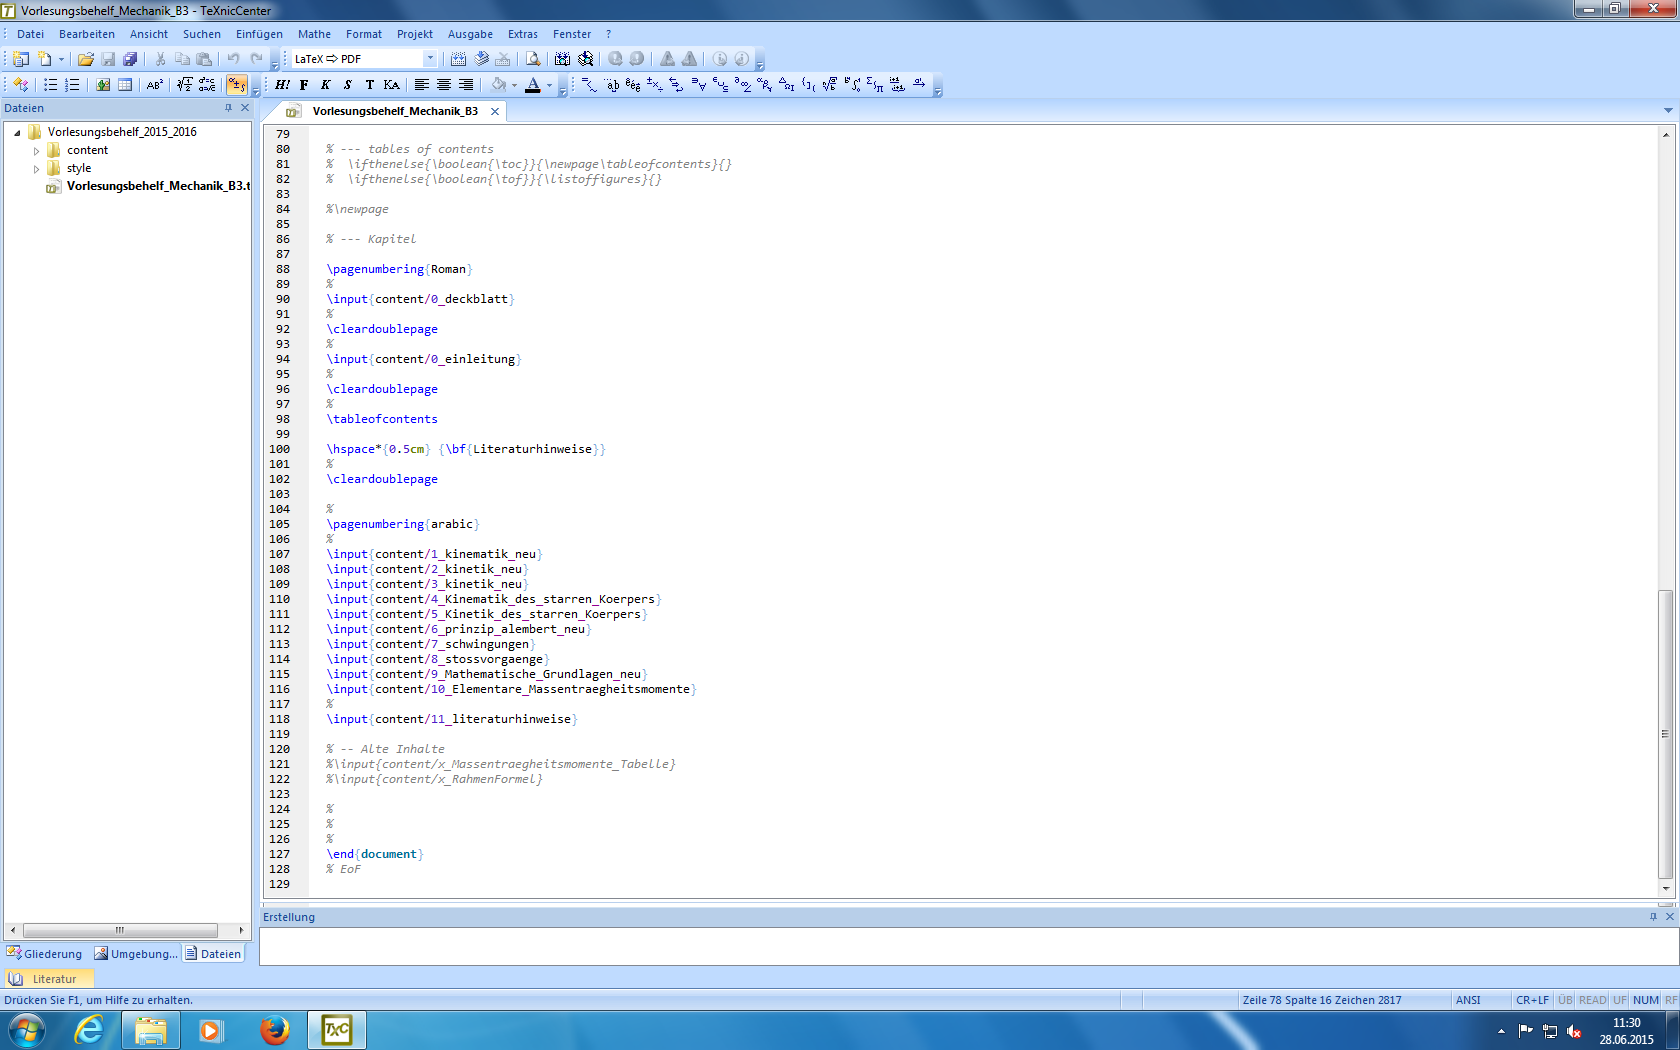
\includegraphics[width=\textwidth]{1_fsMain.png}
  \caption{Der eigentliche Kern von \twrite{Vorlesungsbehelf\_Mechanik\_B3.tex}.
    Oben werden Deckblatt und Einleitung geladen, während im unteren Block alle
    Kapitel eingefügt werden.}
  \label{fig:fsmain}
\end{figure}

\newpage
\section{\"{U}bungsbl\"{a}tter}

Wie bereits im ersten Kapitel erwähnt, werden alle drei übungsbezogenen 
Dokumente (Angaben, Durchgerechnete und Lösungen) aus dem file 
\twrite{Aufgaben.tex} erstellt. Es wird explizit darauf hingewiesen, dass die 
Funktionsweise bei den Übungsblättern ewas anders als bei der Formelsammlung 
ist.

Das Wichtigste zum Verständnis ist, dass in \twrite{Aufgaben.tex} die Variable
(bzw. eigentlich das Kommando) \texcode{\textbackslash myVar} mittels
\texcode{\textbackslash newcommand\{\textbackslash myVar\}\{X\}} definiert ist.
Je nachdem welcher Wert für \texcode{X} eingesetzt wird, wird ein anderes
Dokument kompiliert. Alle möglich Werte von \texcode{X} sind im \TeX-Code an 
dieser Stelle mit Kommentaren beschrieben, und in folgender Tabelle werden nur 
noch die wichtigsten Werte angeben.

\begin{tabularx}{\textwidth}{l|X}%| disable odd look in emacs
  Kommando  & Erzeugtes Dokument \\
  \hline
  \texcode{\textbackslash newcommand\{\textbackslash myVar\}\{1\}}
  & Angaben zu den Aufgaben für Mechanik B3 (Baumechanik 3), Dynamik VT\\
  \hline
  \texcode{\textbackslash newcommand\{\textbackslash myVar\}\{10\}}
  & Angaben zu den Aufgaben für Mechanik - Dynamik\\
  \hline
  \texcode{\textbackslash newcommand\{\textbackslash myVar\}\{3\}}
  & Lösungen (alle Studienrichtungen)\\
  \hline
  \texcode{\textbackslash newcommand\{\textbackslash myVar\}\{5\}}
  & Durchgerechnete Beispiele (alle Studienrichtungen)
\end{tabularx}

Die erzeugten Dokumente bei \texcode{X}=1 und \texcode{X}=10 weichen nur im 
Deckblatt voneinander ab (der Wert 10 ist hierbei als \glqq{}eins-null\grqq{} 
zu verstehen).

\newpage
\begin{center}
\large{\twrite{Aufgaben.tex}}
\end{center}

\begin{tabularx}{\textwidth}{l|X}%| disable odd look in emacs
  Kommando & Erklärung\\ \hline\hline
  % preambel
  \texcode{\textbackslash input \{Basisdaten/style/preambel\}}
  & Lädt die preambel. Im Gegensatz zur Formelsammlung gibt es keine
    Unterscheidung zwischen ein- und zweiseitigem Ausdruck. Es gilt hier auch,
    dass die preambel selbst eigentlich nie verändert werden sollte.\\ \hline
  % macros
  \texcode{\textbackslash input \{Basisdaten/style/macro\}}
  & Lädt die Makros. Praktisch ident zur Formelsammlung.
    \\ \hline
  % reference
  & Folgender Abschnitt wird in In \figref{fig:aufgabemain} dargestellt.\\
  % myVar
  \texcode{\textbackslash newcommand\{\textbackslash myVar\}\{X\}}
  & Anhand der Kommentare kann man ablesen, welche Werte \texcode{X}
    annehmen darf und was jeder Wert repräsentiert.\\\\
  % variable
  \texcode{\textbackslash input \{Basisdaten/style/variable\}}
  & Lädt das Dokument \twrite{variable.tex}. Dieses ist sozusagen der Pivot
    in der Erstellung des Dokuments und wird im Folgenden noch genauer
    besprochen.\\\\
  % begin
  \texcode{\textbackslash begin \{document\}}
  & \\
  % deckblatt
  \texcode{\textbackslash myDeckblatt}
  & Fügt das Deckblatt ein, welches in \twrite{variable.tex} definiert wird.  
    \\\\
  % Inhalt
  \texcode{\textbackslash input \{content/0\_einleitung\}}
  & Fügt den Inhalt ein, welcher in \twrite{variable.tex} definiert wird.\\
  % end
  \texcode{\textbackslash end \{document\}}
  &
\end{tabularx}

\begin{figure}[htbp]
  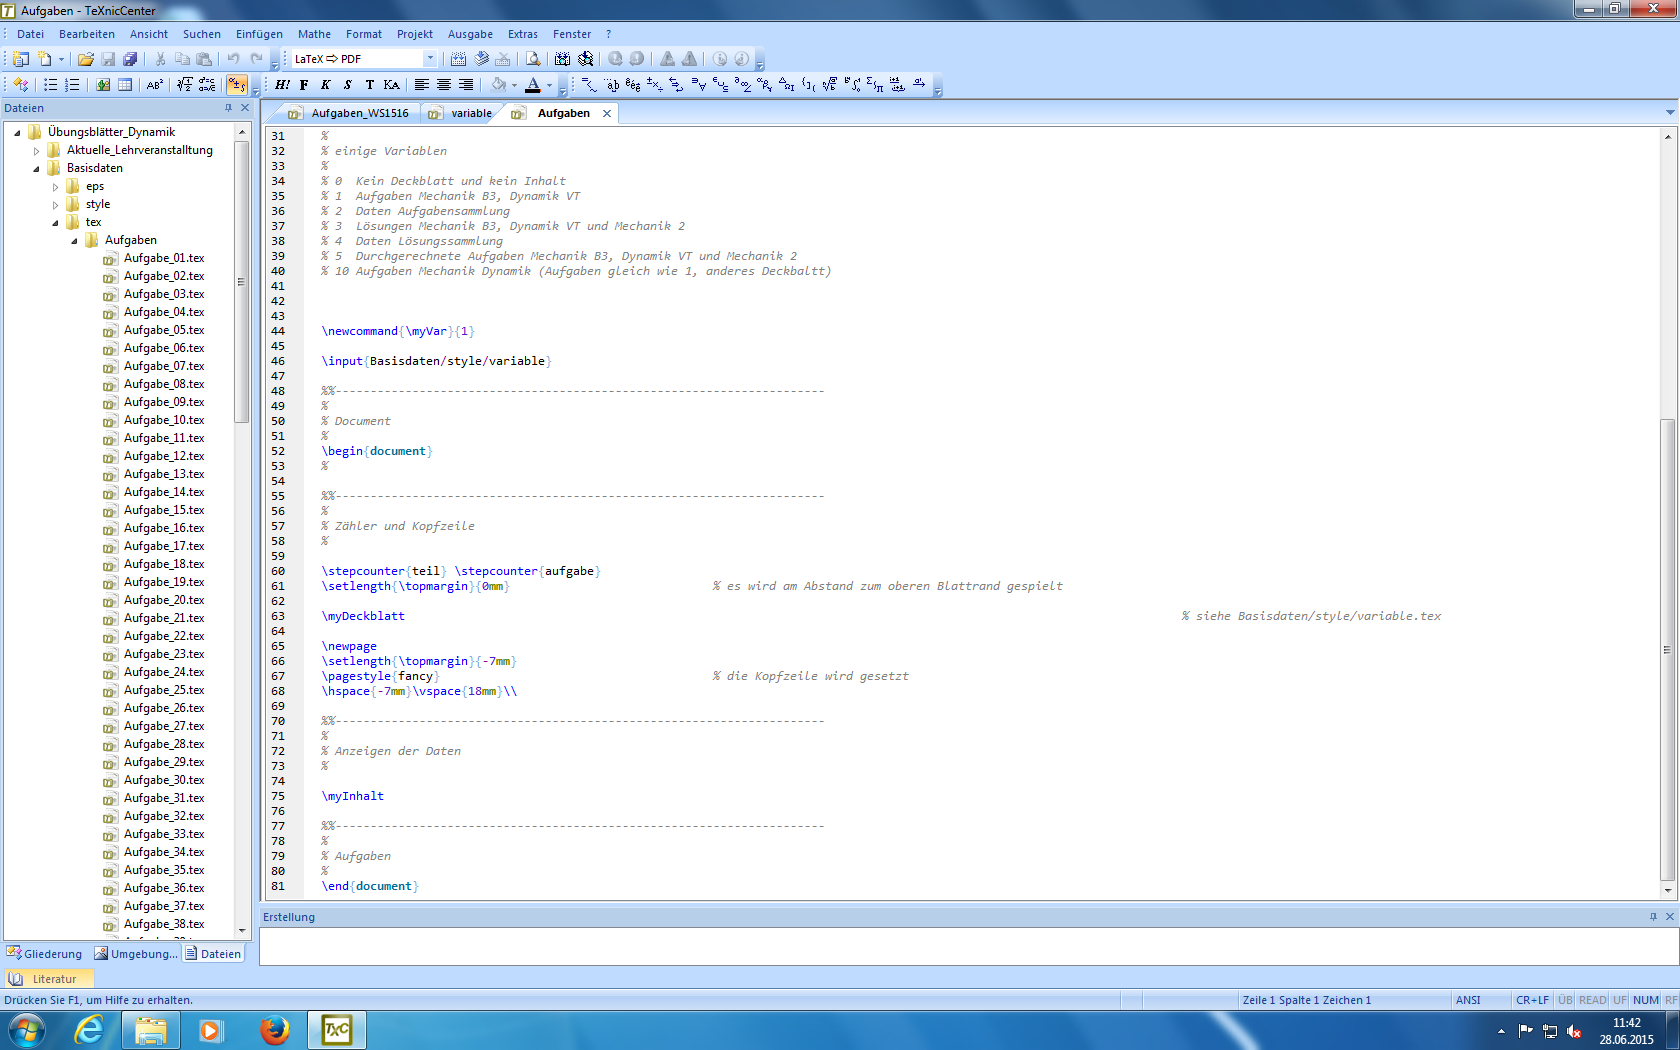
\includegraphics[width=\textwidth]{1_aufgabeMain.png}
  \caption{Der Hauptteil von \twrite{Aufgabe.tex}. Oben wird 
    \texcode{\textbackslash myVar} definiert, wobei die einzelnen Werte im
    Kommentar beschrieben werden. Darunter wird die \twrite{variable} inkludiert
    und weiter unten mit \texcode{\textbackslash myDeckblatt} und 
    \texcode{\textbackslash myInhalt} das eigentliche Dokument eingefügt.}
  \label{fig:aufgabemain}
\end{figure}


\subsection{Dokument \twrite{variable.tex}}

Dieses file ist der Dreh- und Angelpunkt bei den Übungsblättern. Es ist
grundsätzlich in zwei Blöcke gegliedert, die im Folgenden kurz erklärt werden.

\begin{itemize}
 \item {\bf 1. Block}: Im ersten Block werden sehr viele Variablen definitert. 
   Einige davon sind:
   \begin {itemize}
    \item aktuelles Studienjahr
    \item Namen der Studienrichtungen (Bau, Verfahrenstechnik, Mathematik)
    \item Termine (Übungsblattabgabe, Prüfung, Tutorien, \dots)
    \item die Nummern der für die Übungsblattabgabe relevanten Beispiele
   \end{itemize}
   Grundsätzlich kann man beim Durchlesen des \TeX-codes leicht erkennen, was
   welche Variable bedeutet. Beim Wechseln von ein Studienjahr auf das nächste
   sind die meisten Aktualisierungen in genau diesem Block vorzunehmen.
 \item {\bf 2. Block}: Der zweite Block ist in \figref{fig:variable} 
   dargestellt. Hier werden zunächst die Kursnamen (bzw. eigentlich die Namen
   der Dokumente) in Abhängigkeit von \texcode{\textbackslash myVar}
   festgelegt. Dazu wird die \LaTeX-Implementierung des 
   {\bf if-else}-conditionals \texcode{\textbackslash ifthenelse} verwendet.
   Darunter werden die Variablen \texcode{\textbackslash myDeckblatt} und
   \texcode{\textbackslash myInhalt} enstprechend definiert. Diese Variablen
   bestimmen im Endeffekt nur welches Deckblatt und welche Datei der Inhalte
   mittels \texcode{\textbackslash include} geladen werden sollen. Die 
   Deckblätter müssen selbst eigentlich nicht editiert werden, die 
   Dateien der Inhalte aber schon. Die relevanten Dateien werden im Folgenden 
   angeführt.
\end{itemize}

\begin{figure}[htbp]
  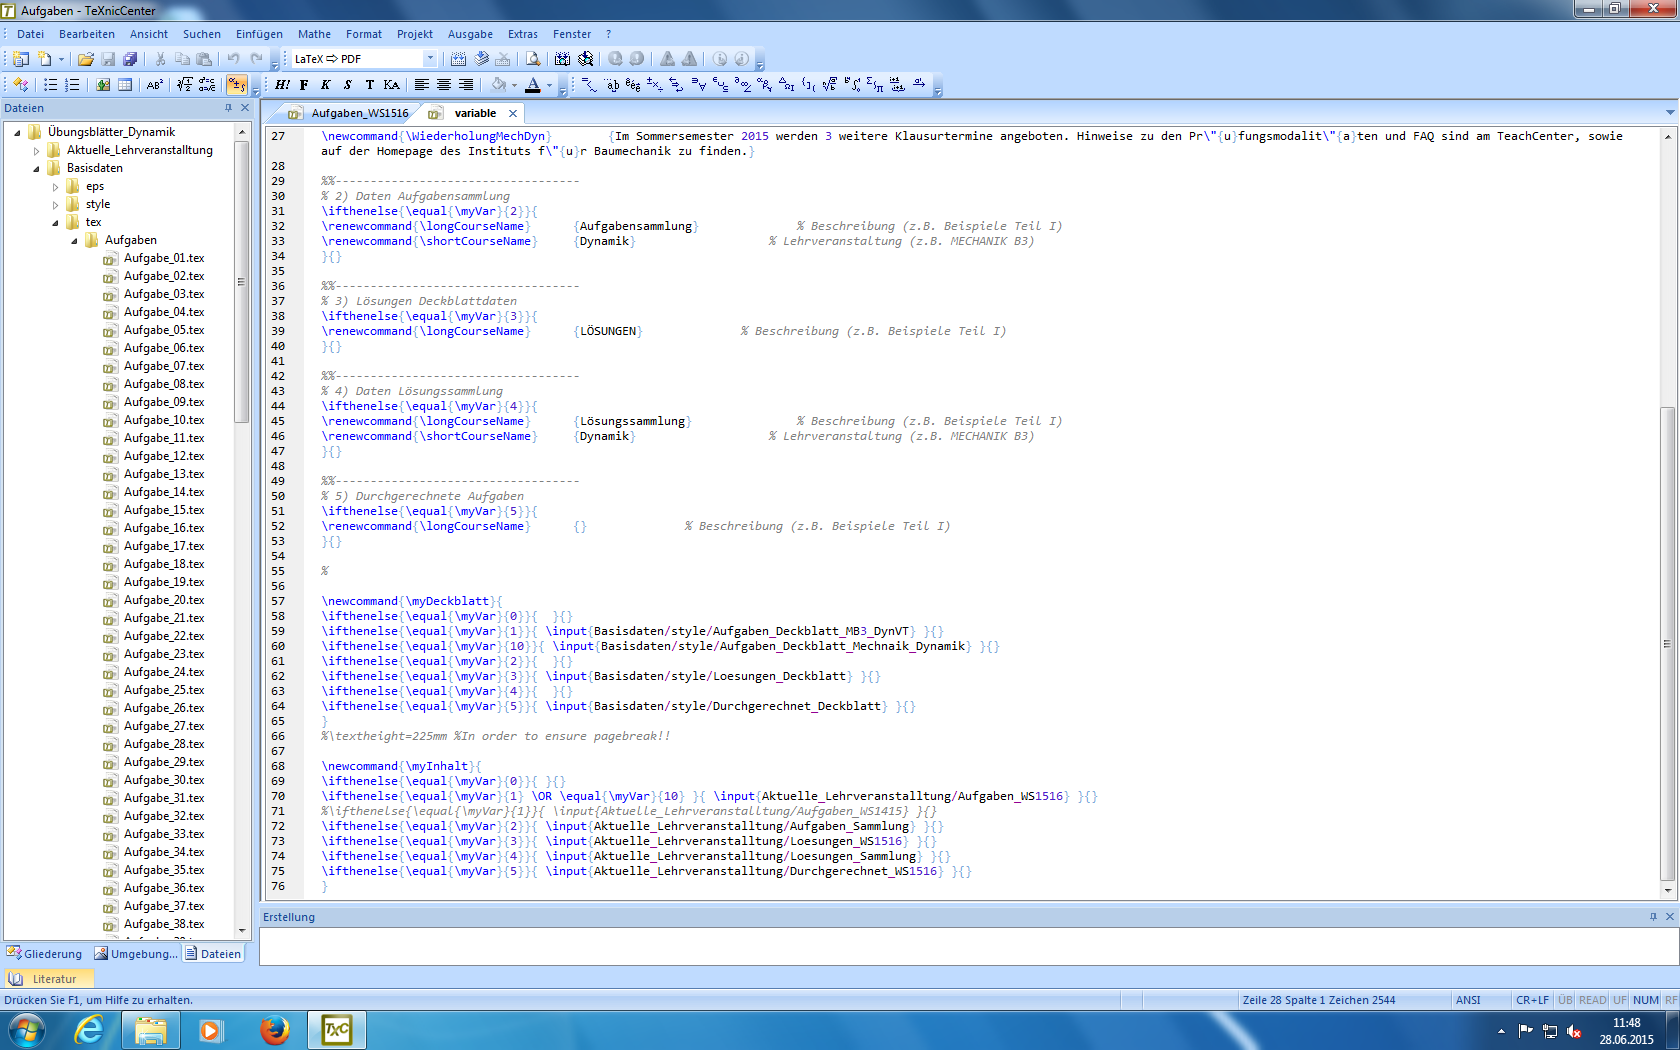
\includegraphics[width=\textwidth]{1_variable.png}
  \caption{Ausschnitt von \twrite{variable.tex}. Oben werden Variablen mit
    den Kursnamen definiert, und unten den Kommandos
    \texcode{\textbackslash myDeckblatt} und \texcode{\textbackslash myInhalt}
    in Abhängigkeit von \texcode{\textbackslash myVar} das richtige Dokument
    zugewiesen. Man kann hier leicht erkennen, dass für die Werte 1 und 10
    unterschiedliche Deckblätter, aber der selbe Inhalt geladen werden
    (man beachte das \texcode{OR} im \texcode{\textbackslash ifthenelse}). Die
    relevanten Inhalte werden in den Fällen 1 (bzw. 10), 3 und 5 geladen.}
  \label{fig:variable}
\end{figure}

\subsection{Dateien der Inhalte (zB. \twrite{Aufgaben\_WSyyzz.tex})}

Die relevanten Inhalte werden in den Fällen 1 (bzw. 10), 3 und 5 geladen.
Diese Dateien sind:

\begin {itemize}
 \item \twrite{Aufgaben\_WSyyzz.tex}
 \item \twrite{Loesungen\_WSyyzz.tex}
 \item \twrite{Durchgerechnet\_WSyyzz.tex}
\end{itemize}

Die meisten anderen Dokumente sind \glqq{}Sammlungen\grqq{}, d.h. es werden
einfach alle Beispiele, die es gibt, geladen. Allerdings werden diese Sammlungen
praktisch nie genutzt.

Die obigen drei Dateien der Inhalte sind alle im Endeffekt gleich aufgebaut. 
Deshalb betrachten wir im Folgenden nur noch die Datei 
\twrite{Aufgaben\_WSyyzz.tex}, da die beiden anderen konzeptuell ident sind.

In \figref{fig:aktaufgabe} ist ein Teil der Datei \twrite{Aufgaben\_WS1516.tex},
dargestellt. Hier werden alle {\tt .tex}-Dateien der Aufgaben 
(\twrite{Aufgabe\_xx.tex}) nacheinander in der vorgschriebenen Reihenfolge 
inkludiert. Hierbei ist Folgendes wichtig: Die \glqq{}interne\grqq{} Nummer 
eines Beispiels (\twrite{Aufgabe\_111.tex} hat die interne Nummer 111) 
hat nichts mit der Reihenfolge des Erscheinens im fertigen Dokument zu tun. 
Wird \twrite{Aufgabe\_111.tex} als drittes durch 
\texcode{\textbackslash include} geladen, so ist es natürlich auch das dritte 
Beispiel. Die korrekte fortlaufende Nummerierung der Beispiele wird durch einen
internen Zähler sichergestellt, der durch \texcode{\textbackslash stepcounter}
nach jedem \texcode{\textbackslash include} inkrementiert wird.

\begin{figure}[htbp]
  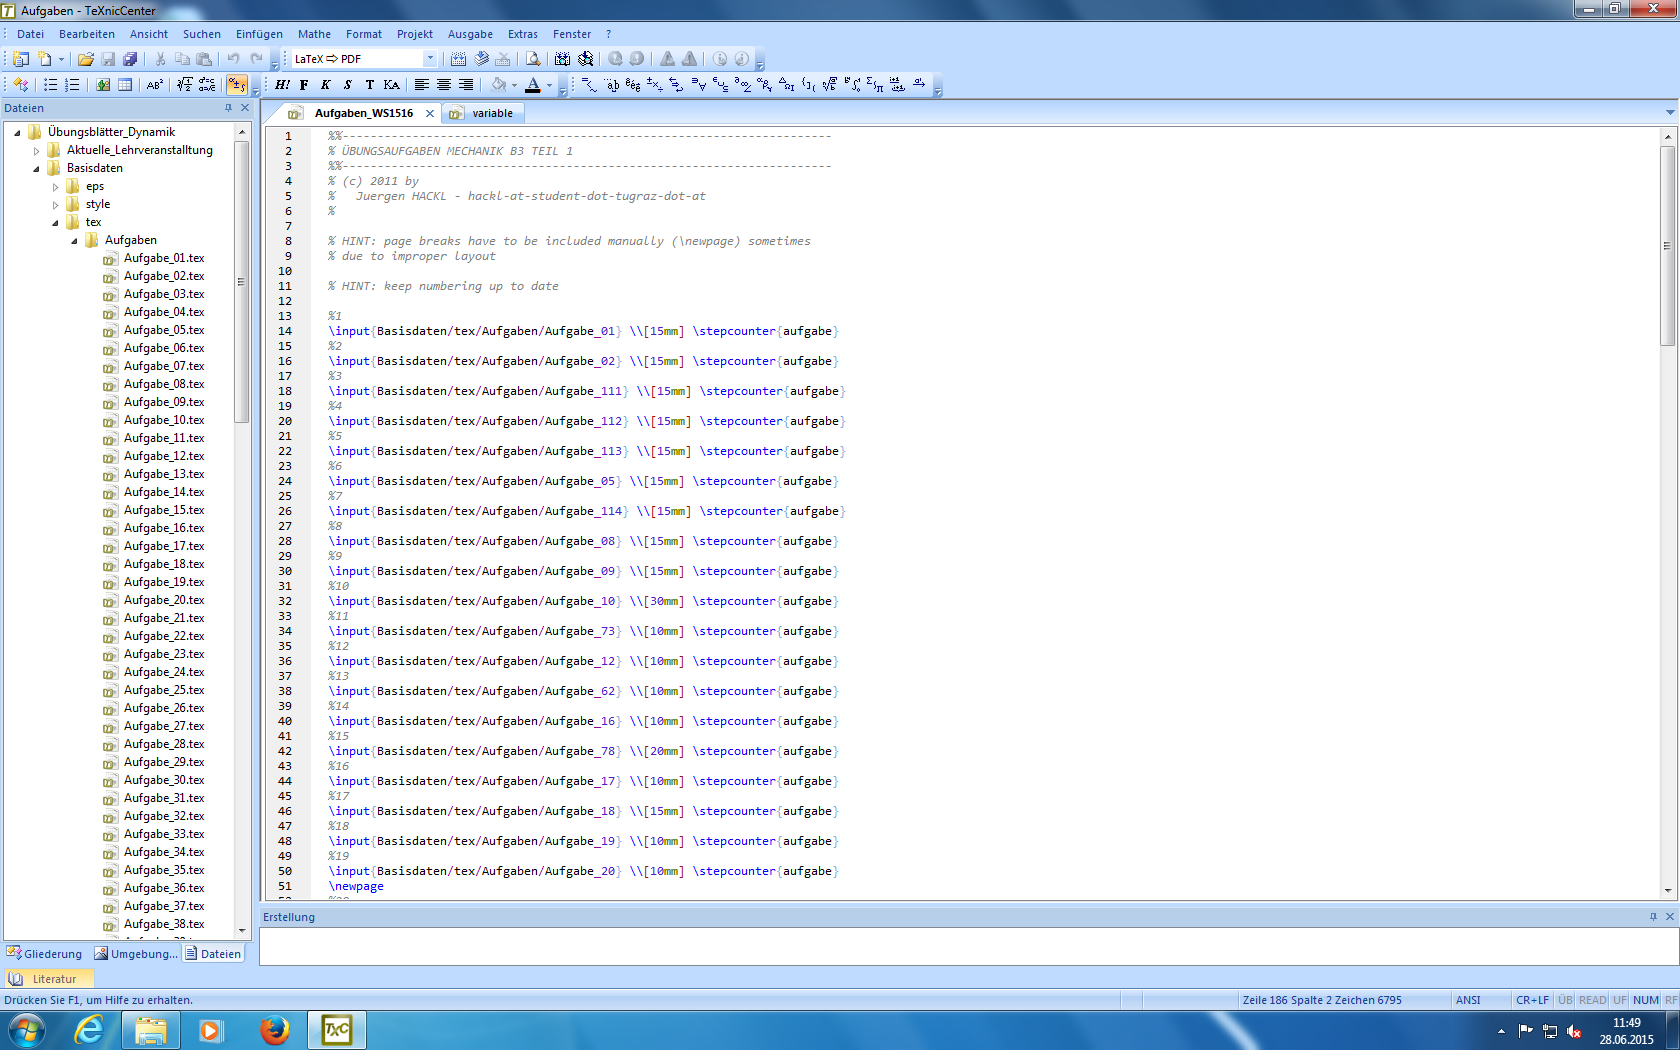
\includegraphics[width=\textwidth]{1_aktAufgabe.png}
  \caption{Ausschnitt von \twrite{Aufgaben\_WS1516.tex}. Die einzelnen
    Aufgaben werden nacheinander eingefügt. Man beachte, dass 
    \texcode{\textbackslash stepcounter} dafür zuständig ist, dass die Beispiele
    im fertigen Dokument richtig (fortlaufend) nummeriert sind.}
  \label{fig:aktaufgabe}
\end{figure}

\subsection{Datei eines Beispiels (z.B. \twrite{Aufgabe\_xx.tex}) }

Hier wird noch exemplarisch die Datei zu einem Beispiel
(\twrite{Aufgabe\_xx.tex}) diskutiert.

In \figref{fig:aufgabe01} wird die Datei \twrite{Aufgabe\_01.tex} dargestellt.
Zuerst wird der Text zur Aufgabe in eine \texcode{\textbackslash minipage}
geschrieben. Es ist darauf zu achten, dass es zwei grundsätzlich verschiedene 
Layouts gibt:

\begin {enumerate}
 \item Der Text (mit den Fragen) geht über die halbe Seitenbreite und die 
   Skizze ist daneben. Hier sind zwei gleich hohe minipages nebeneinander
   angeordnet.
 \item Der Text geht über die gesamte Seitenbreite und darunter sind die Fragen
   neben der Skizze. Hier ist eine kurze minipage über die gesamte Breite und
   darunter zwei gleich hohe minipages nebeneinander angeordnet
   (\twrite{Aufgabe\_01.tex} hat genau dieses Layout).
\end{enumerate}

Nach dem Text wird das Bild eingefügt. Die Beschriftung der Bilder erfolgt 
direkt in \LaTeX{} in der 
\texcode{\textbackslash overpic}-Umgebung mit dem Befehl
\texcode{\textbackslash put(x,y)\{...\}}, wobei \texcode{x} und \texcode{y}
die Koordinaten darstellen. Um das Beschriften leichter zu gestalten, kann man
sich ein Koordinatennetz anzeigen lassen, indem man den Befehl 
\texcode{grid,tics=n} bei der Bildbreite dazuschreibt.
Um im unteren Beispiel ein Koordinatennetz zu zeichnen, muss die 25. Zeile wie
folgt umgeschrieben werden:
\begin{center}
\texcode{\textbackslash begin\{overpic\}[width=6.5cm,grid,tics=5]\{Grafik\_1\}}
\end{center}
Der Abstand der Netzlinien wurde hier mit 5 gewählt, in manchen Fällen ist aber
10 besser geeignet.

Muss man ein neues Beispiel erstellen, so is es ratsam, ein bestehendes (mit dem
richtigen Layout) zu kopieren und nur den Text, die Fragen und das Bild 
zu ändern.

\begin{figure}[htbp]
  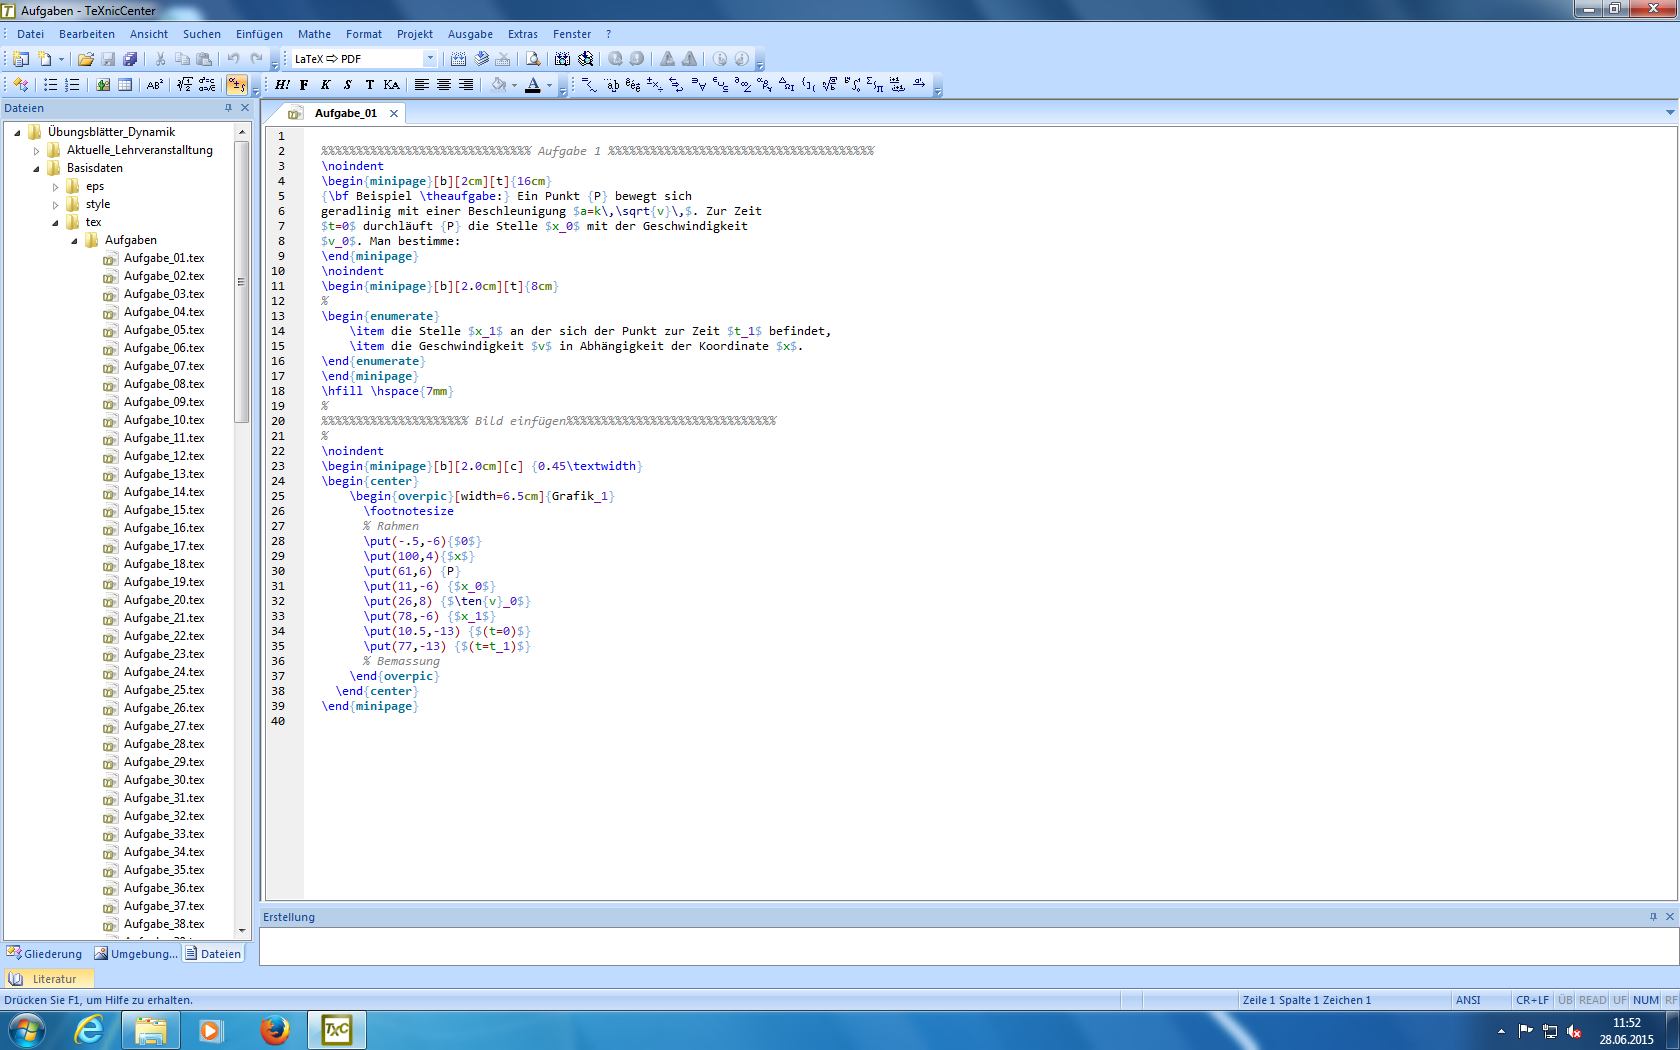
\includegraphics[width=\textwidth]{1_aufgabe01.png}
  \caption{Datei \twrite{Aufgabe\_01.tex}. Hier ist das eigentliche Beispiel
    definiert: Oben steht der Text zur Angabe, gefolgt von den Fragen. Darunter
    wird das Bild geladen und beschriftet.}
  \label{fig:aufgabe01}
\end{figure}

%EOF
%
%% chapter 3 : corel draw
\chapter{Corel Draw}

Beim Arbeiten mit Corel-Draw sind folgende Dinge zu beachten:

\begin{itemize}
  \item Noch viel mehr als bei den \LaTeX-Dokumenten sollte man hier auf
    {\bf copy-and-paste} bauen. Praktisch alle Symbole (Blöcke, Pfeile,
    Auflager, Federn, Dämpfer, etc.) können in den bereits bestehenden 
    {\tt .cdr}-files gefunden werden. Würden eigene Symbole hierfür gezeichnet
    werden, so wäre das neue Bild nicht mehr konsistent mit den restlichen.
  \item Beim Abspeichern der {\tt .cdr}-files sollte man darauf achten, diese
    in {\bf Version 14} abzuspeichern. Dies rührt daher, dass die 
    Corel-Draw-Installation eines Rechners in der Institutsbibliothek nur bis zu
    Version 14 kompatibel ist. Arbeitet man auf dem anderen Rechner hat man 
    darauf achten, dass dieser standardmäßig in höheren Versionen speichert.
  \item Die Nummerierung der Beispiele in der Formelsammlung (z.B.
    \twrite{C01.cdr}, etc.) geschieht zwar ohne wirkliches Muster, ist aber 
    keinesfalls beliebig! Dies soll an folgendem Beispiel erklärt werden: 
    Angenommen im Ordner des dritten Kapitels
    (\twrite{3\_kinetik eines Systems von MP}) befinden sich die Dateien 
    \twrite{C16.cdr}, \twrite{C17.cdr} und \twrite{C18.cdr}. Muss man nun in 
    diesem Kapitel ein neues Bild einfügen, so läge es nahe dieses mit der 
    Nummer19 (\twrite{C19.cdr}) auszustatten. Nun kann es aber durchaus sein, 
    dass in  Kapitel 6 (\twrite{6\_schwingungen}) bereits ein Bild mit dem Namen
    \twrite{C19.cdr} existiert. Problematisch wird das Ganze, wenn
    man nun das Bild als {\tt .eps} exportiert: Zumal die {\tt .eps}-files
    aller Kapitel in dem selben Ordner gespeichert sind, würde man das alte 
    überschreiben.\newline
    Um festzustellen, ob ein Name in Verwendung ist oder nicht, kann 
    Folgendes gemacht werden: Man erstellt das {\tt .cdr} mit dem gewünschten 
    Namen und versucht es gleich als {\tt .eps} zu exportieren. Wenn man jetzt 
    die  Warnung bekommt, dass ein {\tt .eps} mit diesem Namen bereits
    existiert, weiß man, dass der Name schon vergeben ist, bricht die 
    Exportierung ab und sucht einen neuen Namen. Dies ist der Grund wieso die 
    Bezeichnung der Bilder in der Formelsammlung eher undurchsichtig ist: 
    Teilweise werden Indizes verwendet (z.B. \twrite{C19\_a.cdr}) oder auch der
    erste Buchstabe geändert (z.B. \twrite{D19.cdr}).
\end{itemize}

Im Folgenden wird noch auf ein paar Funktionen von Corel Draw eingegangen, die
sich vielleicht nicht sofort erschließen, aber sehr hilfreich sind.

\section{Objekteigenschaften}

Eine der wichtigsten Funktionen sind die Objekteigenschaften. Sie können durch
einen Rechtsklick, gefolgt durch anwählen des Buttons \twrite{Eigenschaften}
angezeigt werden. Alternativ kann man sie auch mit der Tastenkombination
\twrite{Alt + Enter} einblenden. Es gibt hier zwei wichtige Reiter, die im
Folgenden beschrieben werden:

\begin{itemize}
  \item {\bf Füllung} (Farbtopf-Symbol):\\
    Wie der Name schon sagt, kann hier die Farbe und der Verlauf der Füllung
    eingestellt werden (es gibt auch die Option {\tt keine Füllung}). Unter
    \twrite{Erweitert} findet man spezielle Muster, die aber eigentlich nicht
    gebraucht werden.
  \item {\bf Umriss} (Füllfeder-Symbol):\\
    Hier kann man einerseits die Stärke und Farbe der Linien festlegen,
    andererseits können aber auch die Pfeilspitzen editiert werden. Unter
    \twrite{Erweitert} findet man folgende Optionen: Rechts oben können die
    Pfeile an beiden Enden mit \twrite{Optionen} verändert werden. Neben
    Befehlen wie {\tt Bearbeiten} oder {\tt Löschen}, gibt es auch das
    Kommando {\tt Tauschen}, welches die Pfeilspitzen der beiden Enden
    vertauscht. Dies ist nützlich, wenn man bei gekrümmten Pfeilen (die z.B.
    Momente oder Winkelgeschwindigkeiten repräsentieren) den Drehsinn
    ändern möchte.
\end{itemize}

In \figref{fig:objarrow} werden beide Reiter in einer Grafik dargestellt.

\begin{figure}[htbp]
  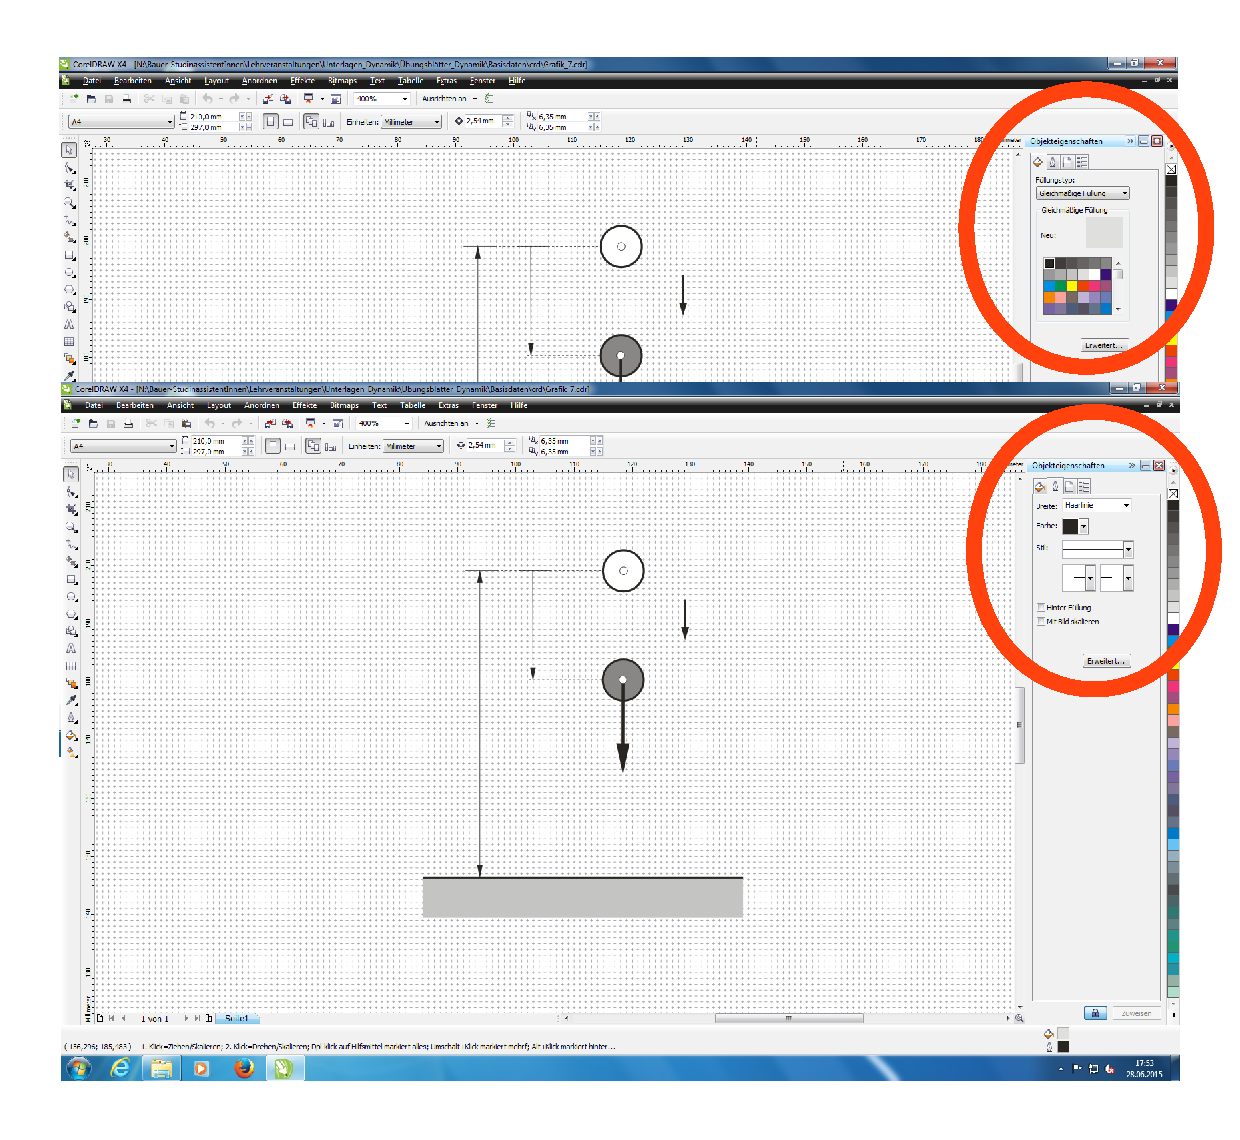
\includegraphics[width=\textwidth]{2_objeigen.pdf}
  \caption{Objekteigenschaften: {\bf Füllung} (oben) und {\bf Umriss} (unten).}
  \label{fig:objarrow}
\end{figure}

\clearpage
\section{Rotation}

Um ein Objekt zu drehen muss man es auswählen und dann noch einmal auf das
Objekt klicken. Es werden gekrümmte Pfeilchen an den Ecken eingeblendet und
der {\bf Rotationspunkt} (dieser ist äquivalent zum mechanischen Momentanpol
einer Bewegung) wird angezeigt. Dieser ist durch einen Kreis mit einem Punkt
darin gekennzeichnet und kann in \figref{fig:rot} beobachtet werden.
Der Rotationspunkt lässt sich beliebig verschieben, was sehr nützlich ist. 
Das Objekt wird gedreht indem man einen der gekrümmten Pfeilchen anwählt und 
das Objekt herumzieht. Alternativ kann in der obigen Aktionsleiste auch der 
Drehwinkel numerisch eingegeben werden.

\begin{figure}[htbp]
  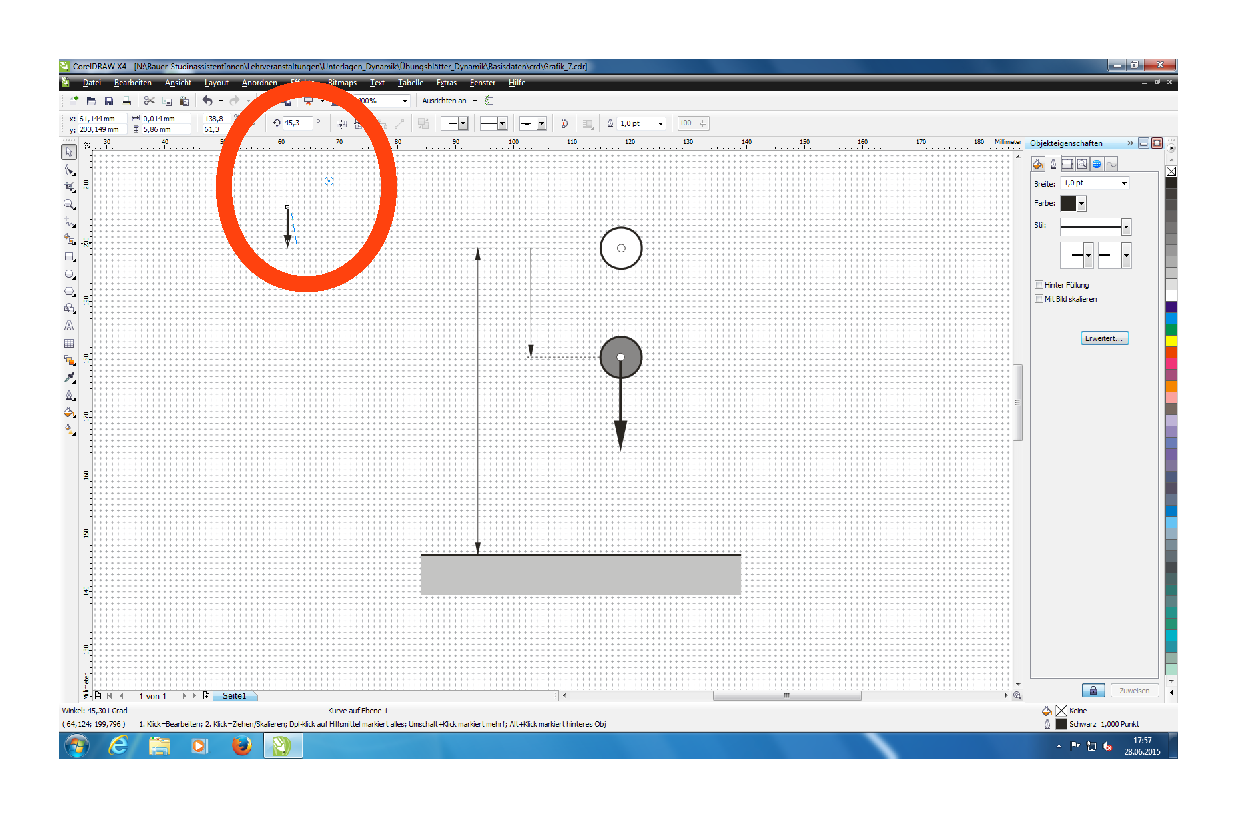
\includegraphics[width=\textwidth]{2_rot.pdf}
  \caption{Rotieren eines Objekts. Man beachte den Rotationspunkt (Momentanpol 
    der Bewegung). In dem durch die Ellipse markierten Bereich befindet sich 
    auch die manuelle Eingabe des Drehwinkels in der Aktionsleiste 
    (ganz oben in der Ellipse).}
  \label{fig:rot}
\end{figure}

\newpage
\section{Hilfsmittel \twrite{Form}}

Das Hilfsmittel \twrite{Form} dient, wie der Name schon suggeriert, zum Ändern
der Form eines Objekts. Es befindet in der linken Aktionsleiste, relativ weit
oben (siehe \figref{fig:form}). Das Tool wird vor allem dazu gebraucht, um bei
Freiformen die Kontrollpunkte der Bezierkurven zu verschieben.

\begin{figure}[htbp]
  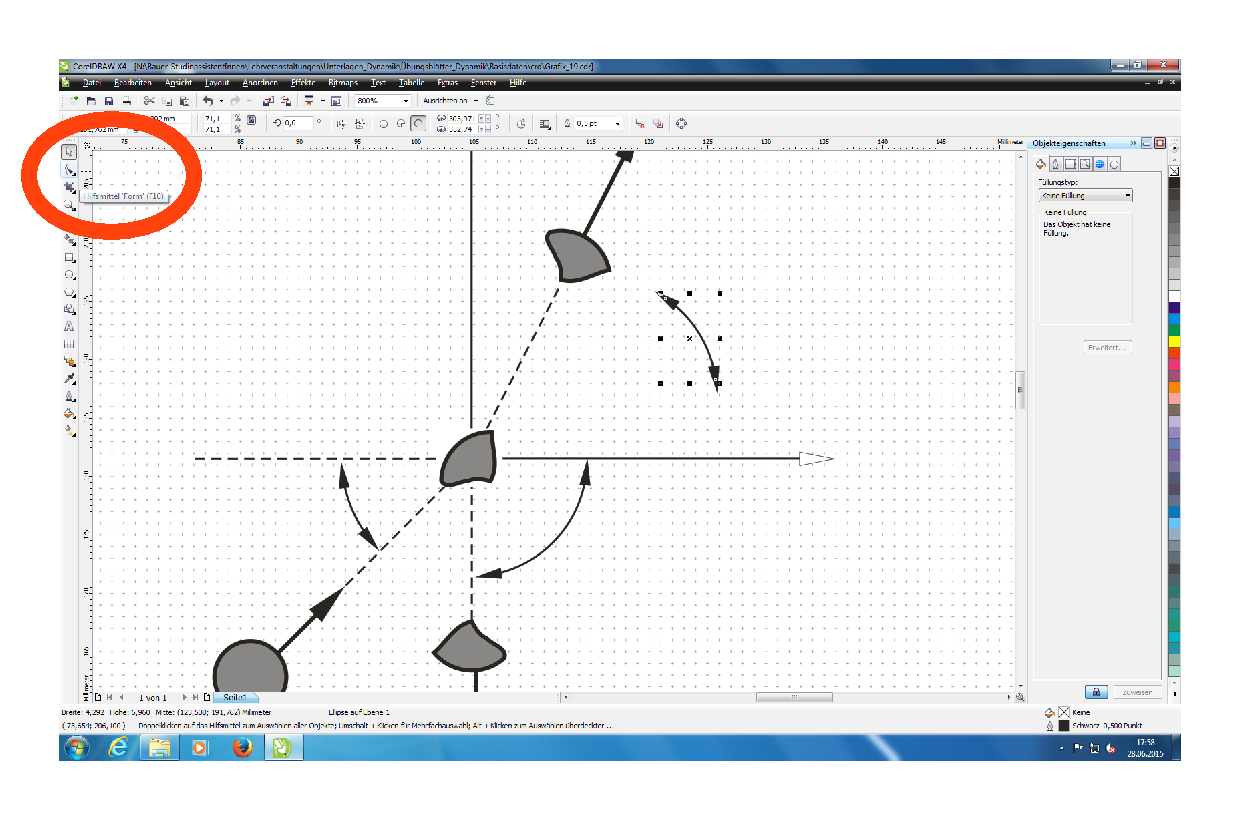
\includegraphics[width=\textwidth]{2_form.pdf}
  \caption{Tool Form.}
  \label{fig:form}
\end{figure}

Ein weiterer wichtiger Anwendungsfall von \twrite{Form} tritt im Zusammenhang
mit Kreissektoren auf. Grundsätzlich wird es dazu verwendet, um den 
Öffnungswinkel zu verändern. Es ist jedoch wichtig wo der Mauscursor
positioniert ist, wenn die Maustaste losgelassen wird: Befindet sich der Cursor
innerhalb des Kreissegments, so wird das eigentliche Segment gezeichnet 
(berandet durch einen Kreisbogen und zwei Geraden). Dieser Sachverhalt wird in 
\figref{fig:circlein} dargestellt. Ist aber der Cursor außerhalb des Segments,
wenn die Maustaste losgelassen wird, so wird nur der Kreisbogen gezeichnet,
inklusive Pfeilchen (sofern vorhanden), siehe \figref{fig:circleout}. 
Erstere Option eignet sich also, um echte Kreissegmente 
(\glqq{}Tortenstücke\grqq{}) zu zeichnen, während letztere gebraucht wird, um 
Winkel einzuzeichnen.

\begin{figure}[htbp]
  \begin{center}
  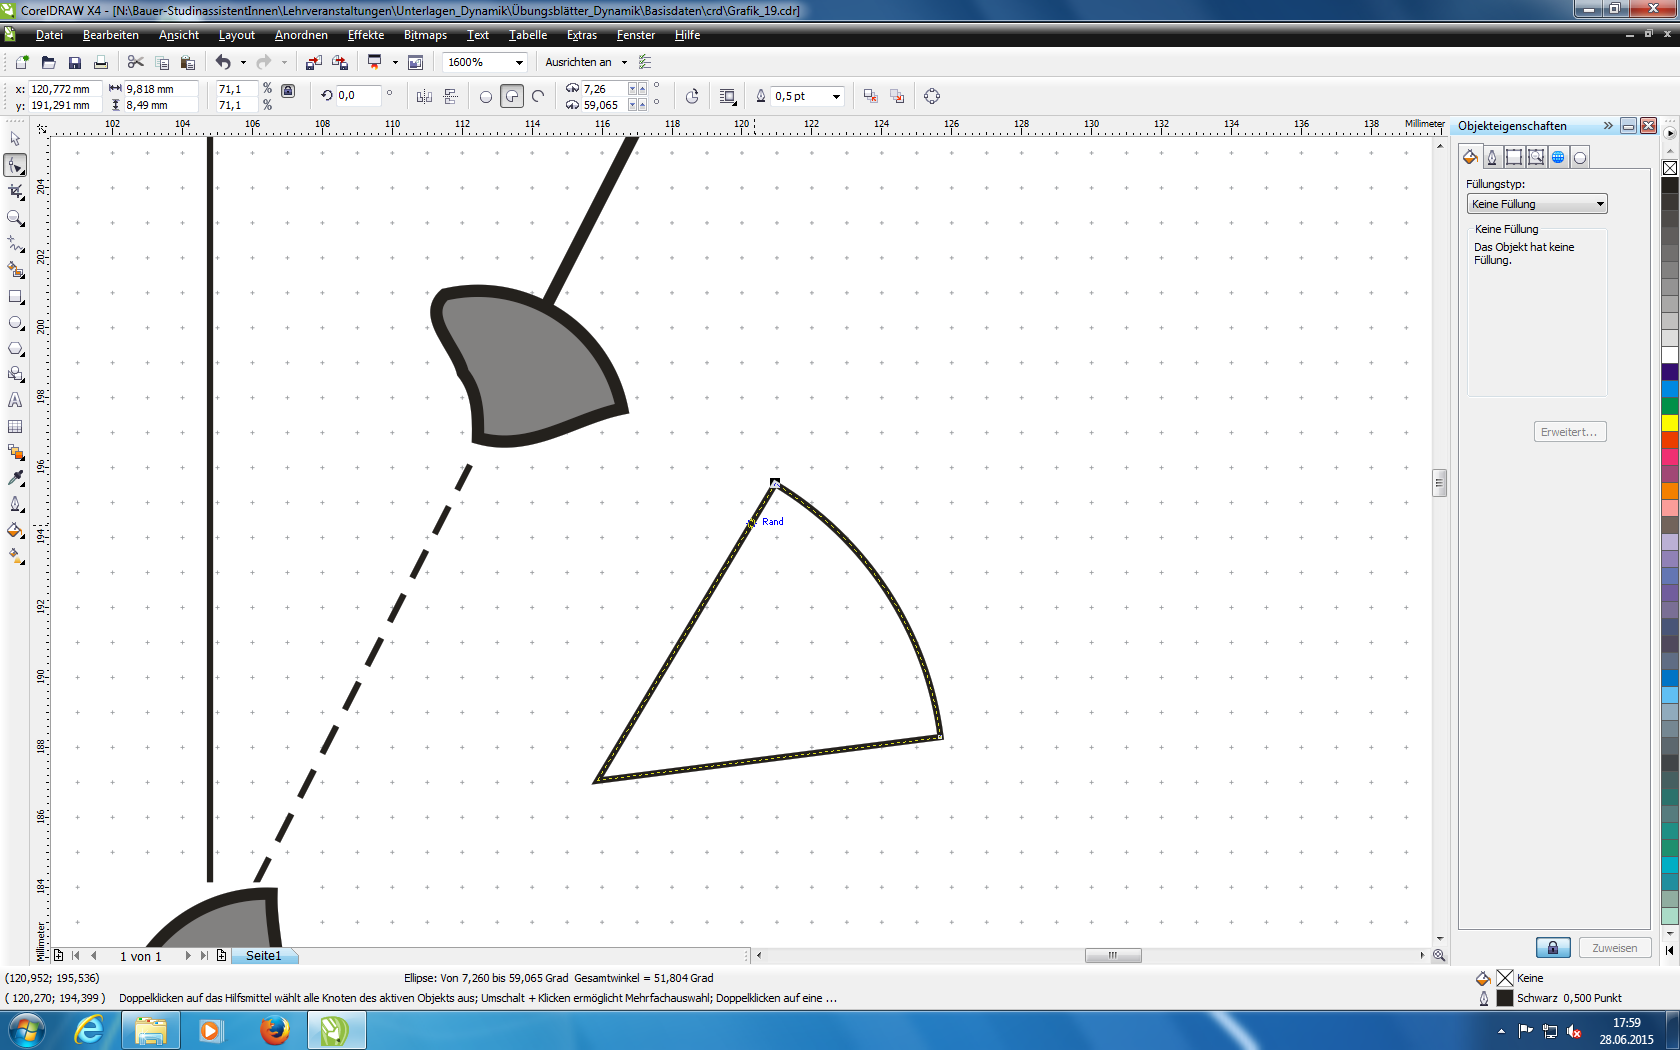
\includegraphics[width=.9\textwidth]{2_circle_in.png}
  \end{center}
  \caption{Tool \twrite{Form} angewendet auf einen Kreissektor. Der Cursor wird
   innerhalb des Segments losgelassen, wodurch das volle Segment (ohne
   Pfeilspitzen) gezeichnet wird.}
  \label{fig:circlein}
\end{figure}


\begin{figure}[htbp]
  \begin{center}
  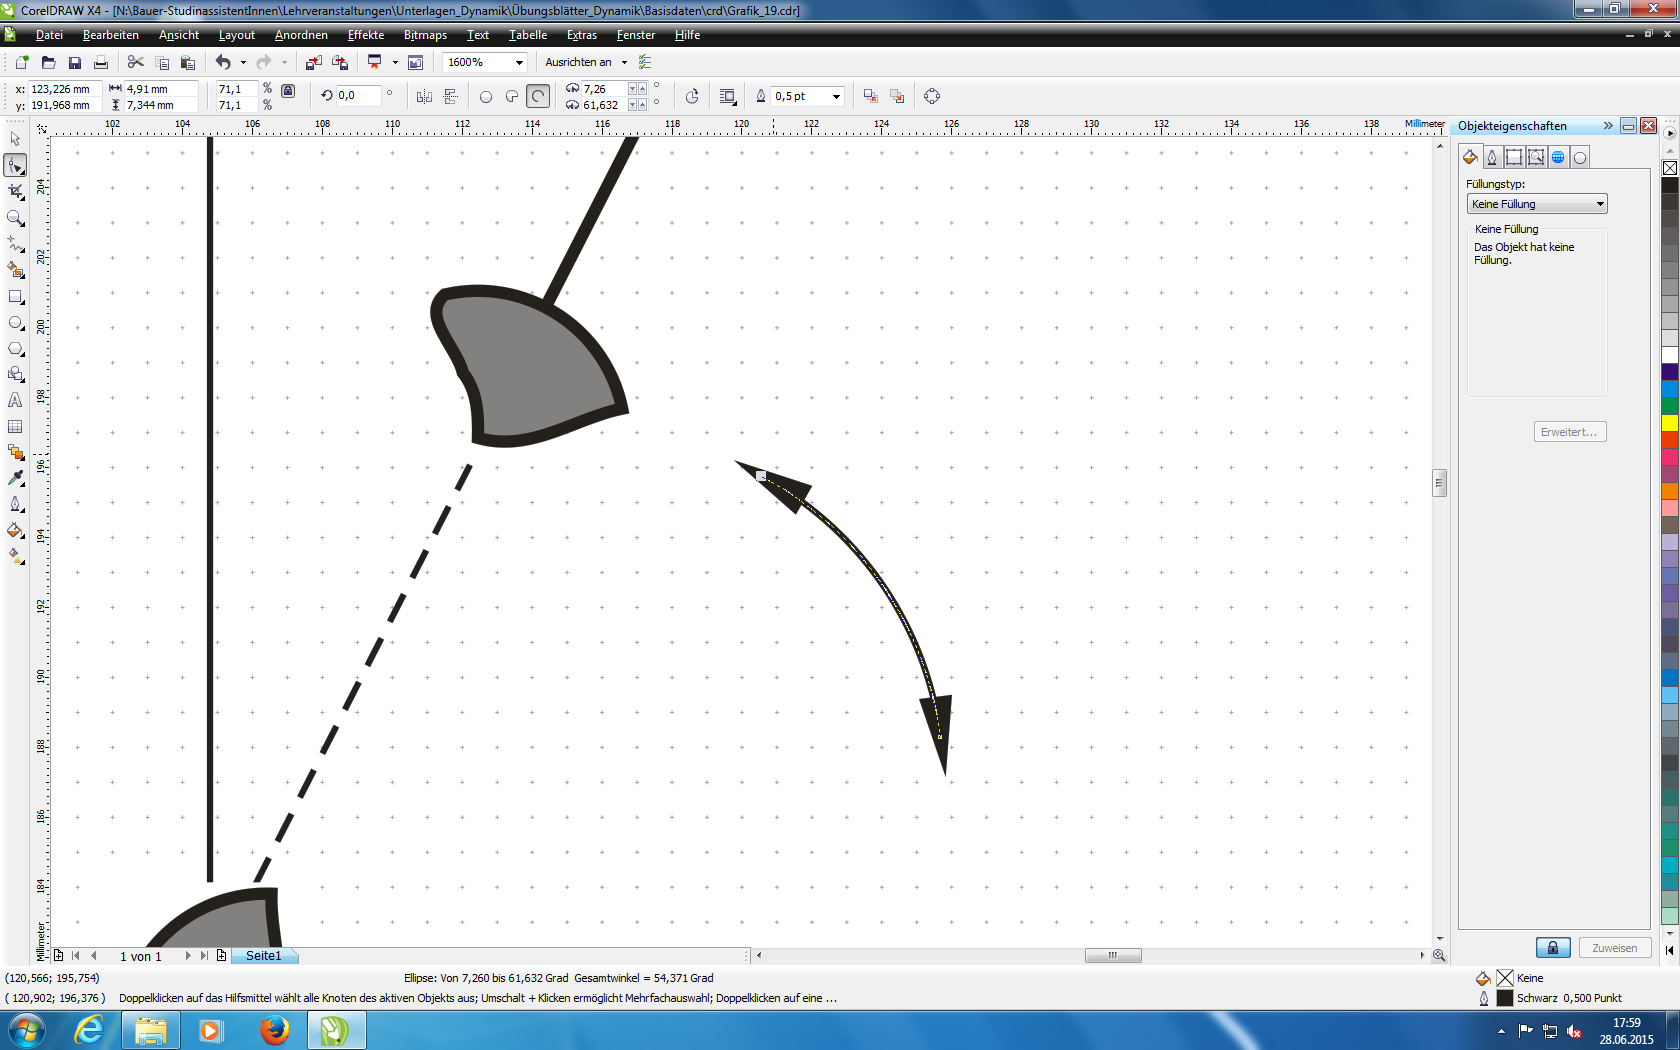
\includegraphics[width=.9\textwidth]{2_circle_out.png}
  \end{center}
  \caption{Tool \twrite{Form} angewendet auf einen Kreissektor. Der Cursor wird
   außerhalb des Segments losgelassen, wodurch nur der Kreisbogen (mit
   eventuell vorhandenen Pfeilspitzen) gezeichnet wird.}
  \label{fig:circleout}
\end{figure}

%EOF
%
% chapter 3 : teach center
\chapter{Teach Center}

Auf der offiziellen Seite des Teach Centers bietet die TU Graz einige Tutorials 
an:\linebreak\url{\tctugraz}\linebreak Viele der Möglichkeiten des TC
werden im Rahmen der Lehrveranstaltung aber nicht benötigt (z.B. Foren,
Umfragen, etc.), weshalb hier die wirklich gebrauchten Funktionen nochmals
skizziert werden.

Das TC funktioniert grundsätzlich recht intuitiv. Man loggt sich ganz normal 
ein, hat aber mehr Rechte als der reguläre Studierende. Zuerst wird auf die
allgemeine Handhabung des TC eingegangen und dann die wichtigsten Funktionen 
der vier Reiter \twrite{Schwarzes Brett}, \twrite{Administratives}, 
\twrite{Unterlagen} und \twrite{Lehr- und Lernhilfen} beschrieben.

{\bf Wichtig:} Jedes Fach im TUGonline hat eine eigene Teach Center Gruppe. 
Es gibt eine eige Gruppen für {\tt Mechanik B3}, 
{\tt Dynamik VT}, {\tt Mechanik - Dynamik (VO)} und 
{\tt Mechanik - Dynamik (UE)}. Wird also eine Verlautbarung auf das Schwarze
Brett von {\tt Dynamik VT} gestellt, so muss sie für alle anderen Gruppen
kopiert werden. Analog verhält es sich mit den Unterlagen: Skriptum und
Übungsblätter müssen in alle TC-Gruppen separat hochgeladen werden (natürlich
müssen übungszogene Inhalte nicht in {\tt Mechanik - Dynamik (VO)}
gestellt werden). Die einzige Ausnahme hierbei ist die Anmeldung zur
Übungsblattabgabe, welche nur ein einiziges mal in der Gruppe 
{\tt Baumechanik 3 (Mechanik B3)} erstellt werden muss. Damit aber alle
Studierenden wissen, wo sie sich anzumelden haben, muss in den anderen Gruppen
die Anmeldung verlinkt werden. Wie hier vorgegangen werden sollte, wird im Part
zur Anmeldung zur Übungsblattabgabe detailliert.

\section{Allgemeine Funktionen}

Die allgemeinen Funktionen finden sich, wie in \figref{fig:general} dargestellt,
rechts oben, wobei die einzig wichtigen Punkte \twrite{Administration} und
\twrite{Benutzer} sind.

\begin{figure}[htbp]
\begin{center}
  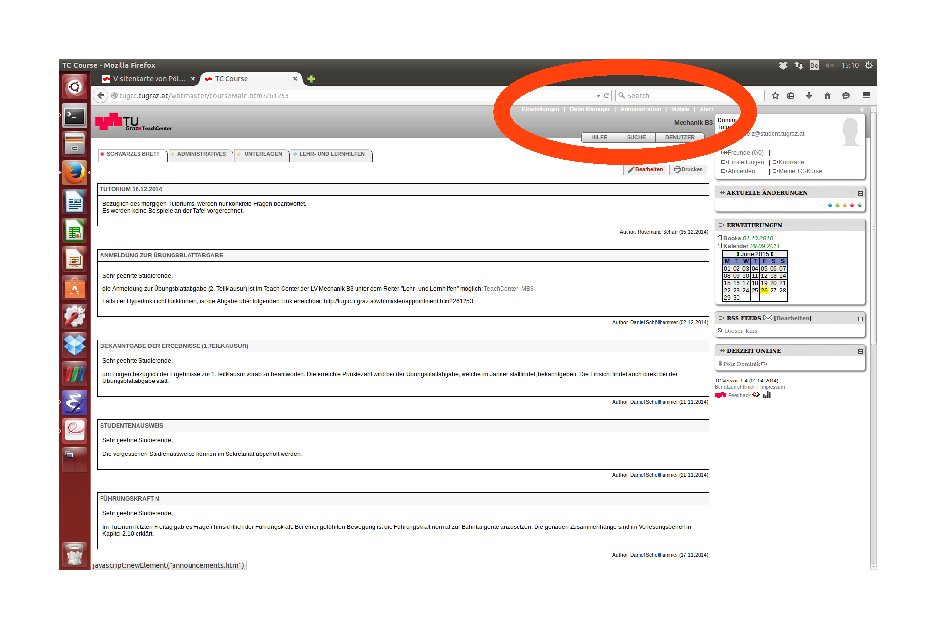
\includegraphics[width=.84\textwidth]{3_general.pdf}
  \caption{ Die allgemeinen Funktionen. In der ersten Zeile ist vor allem 
    \twrite{Administration} und in der zweiten \twrite{Benutzer} relevant.}
  \label{fig:general}
\end{center}
\end{figure}

%Im Folgenden gehen wir auf die wichtigsten Funktionen von
%\twrite{Administration} ein.

\subsection{Administration - Parameter}

Hier können neue \glqq{}Course Tutors\grqq{}, also StudienassistentInnen mit
Schreibrechten, der TC Gruppe hinzugefügt werden. Um dies zu tun, muss in
der Zeile \twrite{Course Tutors} - dargestellt in \figref{fig:params} - 
die TUG-ID des Nutzers hinzugefügt werden, wobei die einzelnen IDs durch ein 
Semikolon getrennt sind. Danach muss die neue Liste unten mit dem Button 
\twrite{Ok} bestätigt werden. Natürlich können auch bestehende Zugriffsrechte 
durch Entfernen der Nutzer-IDs entzogen werden. Alle weiteren Funktionen werden 
praktisch nicht benötigt.

{\bf Herausfinden der TUG-ID:} Loggt man sich ins TC mit seinem Account ein, so
sieht man auf der rechten Seite die Kurskarte und ganz rechts oben seinen Namen.
Man klickt auf diesen und im folgenden Fenster klickt man auf
\twrite{Bearbeiten}. Es öffnet sich ein Fenster, und in der ersten Zeile
steht {\tt Modify Account \grqq{}<ID>\grqq{}}, wobei {\tt <ID>} die gesuchte
ID ist.

\begin{figure}[htbp]
\begin{center}
  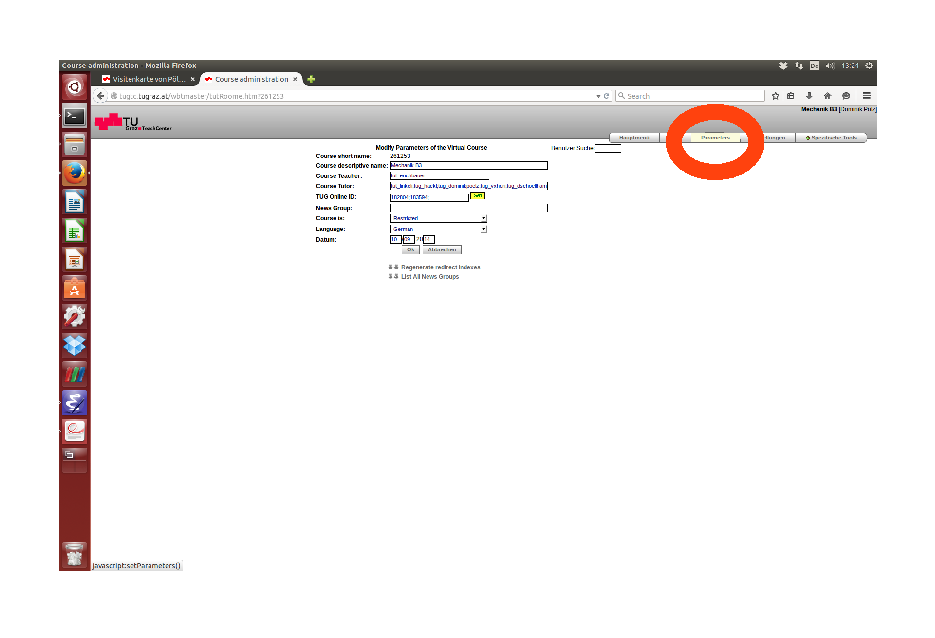
\includegraphics[width=\textwidth]{3_params.pdf}
  \caption{ \twrite{Administration} - \twrite{Parameters} }
  \label{fig:params}
\end{center}
\end{figure}

\subsection{Administration - Einstellungen}

Hier können Funktionen des TC ein- und ausgeschaltet werden, wie beispielsweise
das Forum. Im Allgemeinen müssen aber keine Änderungen vorgenommen werden.

\subsection{Benutzer}

Hier werden die Leserechte an der TC Gruppe geregelt, d.h. alle hier 
eingetragenen Studierende haben Zugriff zur Gruppe. 

\subsubsection{Exportierung Teilnehmerliste}

Um eine Teilnehmerliste aus dem Teach Center in Excel zu exportieren, müssen
folgende Schritte unternommen werden (\figref{fig:export} stellt diesen
Prozess grafisch dar):

\begin{enumerate}
\item Button \twrite{Benutzer}
\item Button \twrite{Liste drucken}
\item Button \twrite{Alle auswählen}
\item Button \twrite{Exportieren} und Button \twrite{CSV exportieren}
\item Im Fenster {\bf ctrl-a} (alles auswählen) und {\bf ctrl-c} (kopieren)
  drücken.
\item In Excel {\bf ctrl-v} (einfügen) drücken. Darauf folgt ein Dialog zur
  Importierung: Hier muss als Trennsymbol (\glqq{}separator symbol\grqq{})
  das Semikolon gewählt werden. In der Vorschau unten kann man dann erkennen,
  dass die Daten in drei Spalten getrennt werden.
\end{enumerate}

\begin{figure}[htbp]
  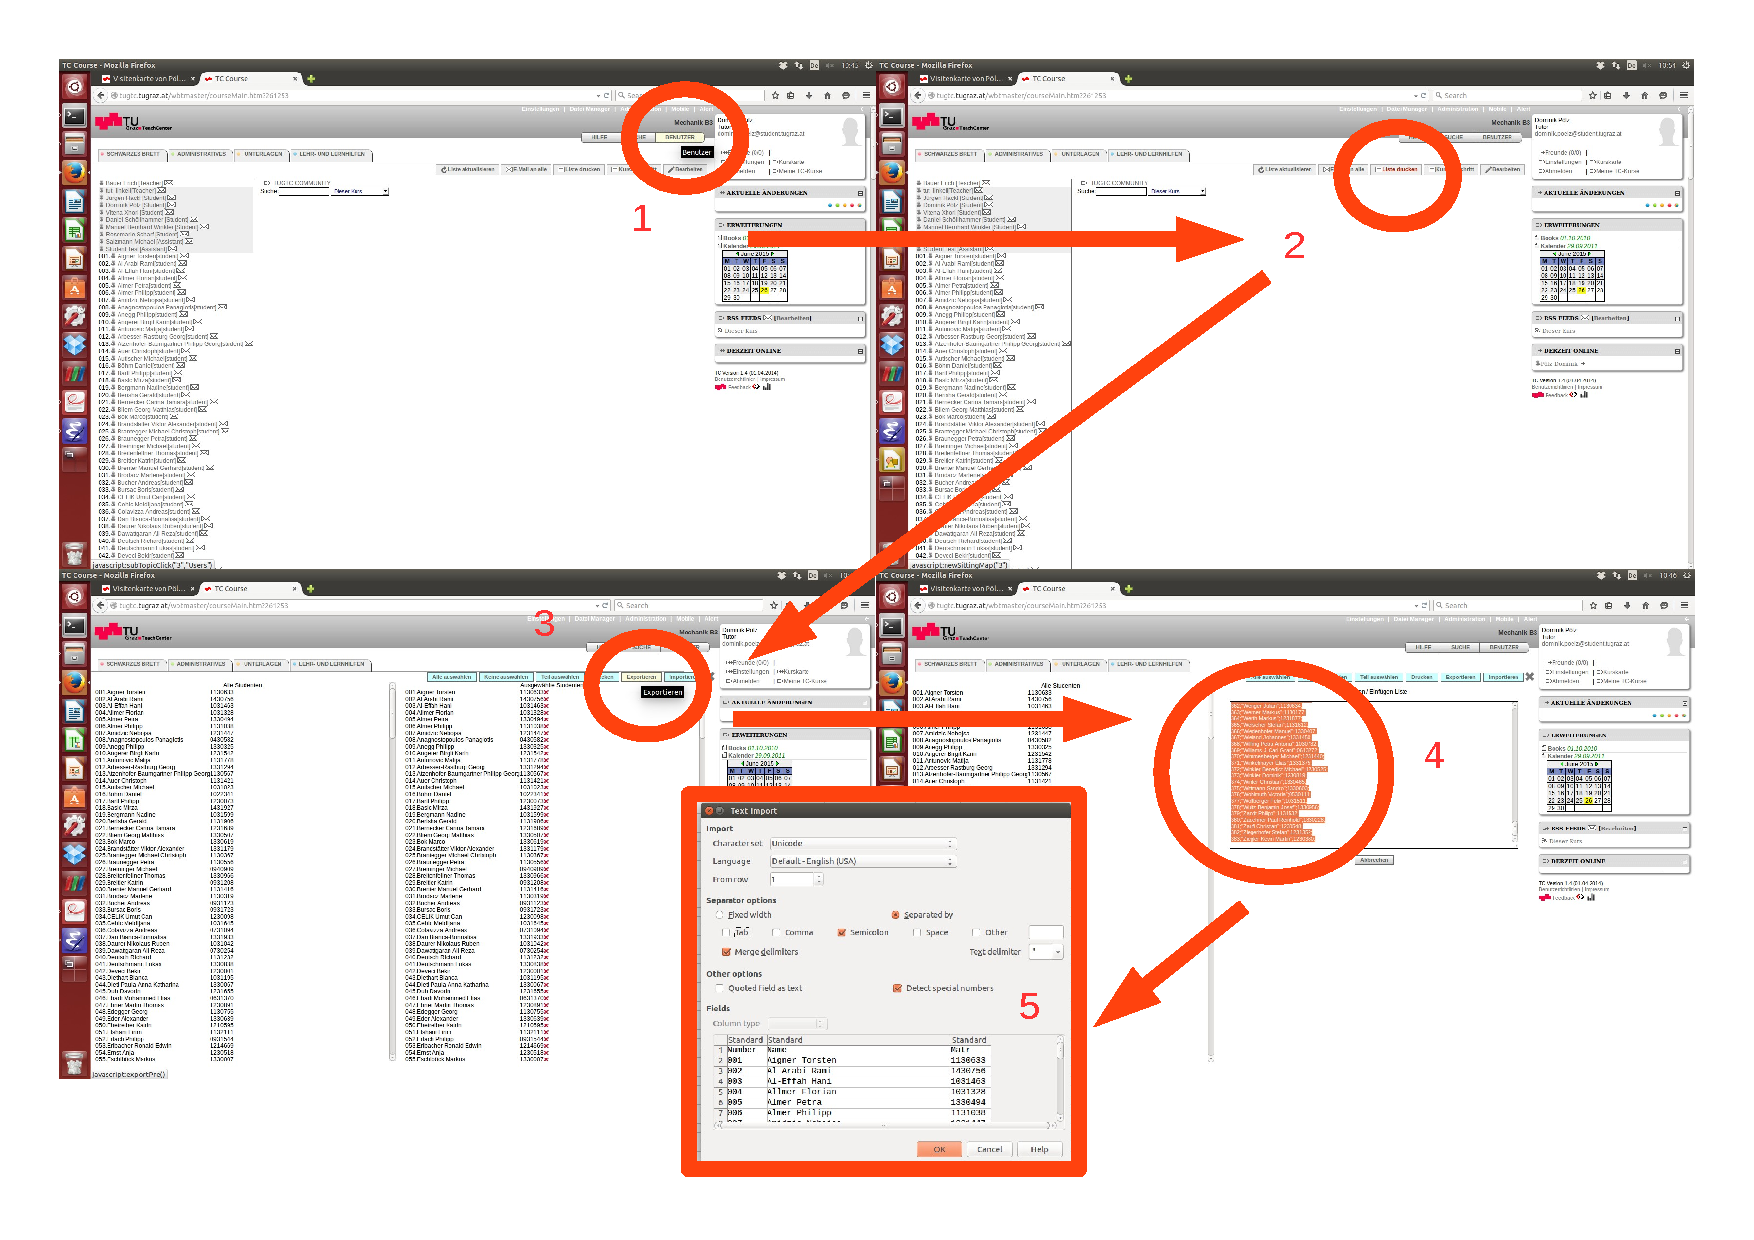
\includegraphics[width=\textwidth]{3_exportList.pdf}
  \caption{ (1) Auswahl Benutzer. (2) Liste drucken. (3) Alle ausw\"{a}hlen und
    exportieren. (4) Gesamten Inhalt kopieren und (5) in Excel einf\"{u}gen,
    wobei das richtige Trennsymbol zu w\"{a}hlen ist.}
  \label{fig:export}
\end{figure}

\subsubsection{Hinzufügen von Studierenden}

Manchmal kommt es vor, dass einzelne Studierende zur Lehrveranstaltung
nachgemeldet werden. Diese haben standardmäßig keine Zugriffsrechte auf das
TC und müssen somit manuell hinzugefügt werden.

Wichtig ist hierbei Folgendes: Das 
\glqq{}Hinzufügen von Studierenden ins TC\grqq{} ist Nichts anderes als eine 
Synchronisierung mit der Liste jener Studentierenden die im TUGonline zur 
Lehrveranstaltung angemeldet sind. Folglich muss man nicht einzelne Studierende
per Hand einfügen, sondern führt einfach einen {\bf refresh} der Liste im TC 
aus.

Um die Liste zu aktualisieren, muss Folgendes gemacht werden.
\begin{enumerate}
\item Button \twrite{Benutzer}
\item Button \twrite{Bearbeiten}
\item Button \twrite{Import}, siehe \figref{fig:import}
\end{enumerate}

{\bf Wichtig:} Dieser Prozess kopiert die aktuelle Liste der zur
Lehrveranstaltung gemeldeten Studierenden des TUGonline und überschreibt die
TC-Liste. Um einen Studierenden also wirklich hinzufügen zu können, muss er/sie
zur Lehveranstaltung gemeldet sein. Studienassistenten haben aber keine Rechte,
um Studierende im TUGonline nachzumelden, und somit muss der Studierende zuerst
vom Sekretariat im TUGonline  nachgemeldet werden, bevor man ihn/sie ins TC
importieren kann.

\begin{figure}[htbp]
  \begin{center}
  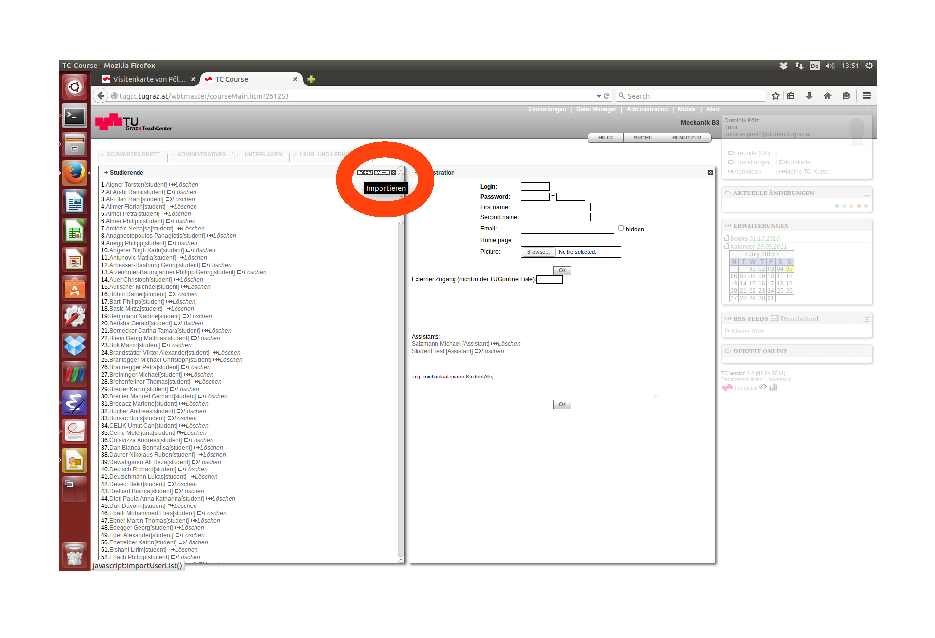
\includegraphics[width=.84\textwidth]{3_import.pdf}
  \caption{ Import der Liste der Studierenden.}
  \label{fig:import}
  \end{center}
\end{figure}

{\bf Anmerkung:} Unter \twrite{Administration} $\to$ \twrite{Spezifische Tools}
(ganz rechts) $\to$ \twrite{Benutzer} kann die Liste der Studierenden ebenfalls
importiert werden. Zusätzlich kann der Import von manuell auf automatisch 
umgestellt werden. Diese Option findet sich in der ersten Zeile, die in etwa
so aussieht:\newline
\texcode{Mechanik B3 [restricted] [Import is Manual]}

Wobei \texcode{Mechanik B3} den Kursnamen der aktuell betrachteten TC Gruppe
darstellt. Durch Klicken auf \texcode{[Import is Manual]} kann auf
\texcode{[Import is Automatic]} umgestellt werden. Es wurde aber bisher
gewünscht, dass der Import {\bf manuell} bleibt, d.h. vor Umstellung auf 
automatischen Import ist in jedem Fall nachzufragen.

\section{Schwarzes Brett}

Hier werden aktuelle Informationen bzw. Ankündigungen hineingeschrieben. Um
einen neuen Beitrag zu erstellen bzw. einen bestehenden zu editieren, müssen
folgende Schritte beachtet werden (siehe dazu \figref{fig:sb}):
\begin{enumerate}
\item Button \twrite{Bearbeiten}
\item Button \twrite{Neu} oder \twrite{Edit}
\end{enumerate}

Daraufhin öffnet sich ein Editor, in dem man den Text schreiben kann. Durch
Klick auf \twrite{HTML Editor} wechselt man auf einen WYSIWYG\footnotemark[1]
-Editor, in dem die HTML-tags automatisch erzeugt werden (wenn man den Text
fertig geschrieben hat, kann man ihn unten mit \twrite{Submit} in den
normalen Editor überspielen). Unten gibt es noch ein paar weitere Optionen,
die man aber meist nicht braucht.

\footnotetext[1]{\glqq{}what you see is what you get\grqq{} - Man sieht das
fertige Ergebnis und keine Kommandos. Auf dem Montitor erscheint nicht
\twrite{<strong>Text</strong>} sondern {\bf Text}.}

\begin{figure}[htbp]
  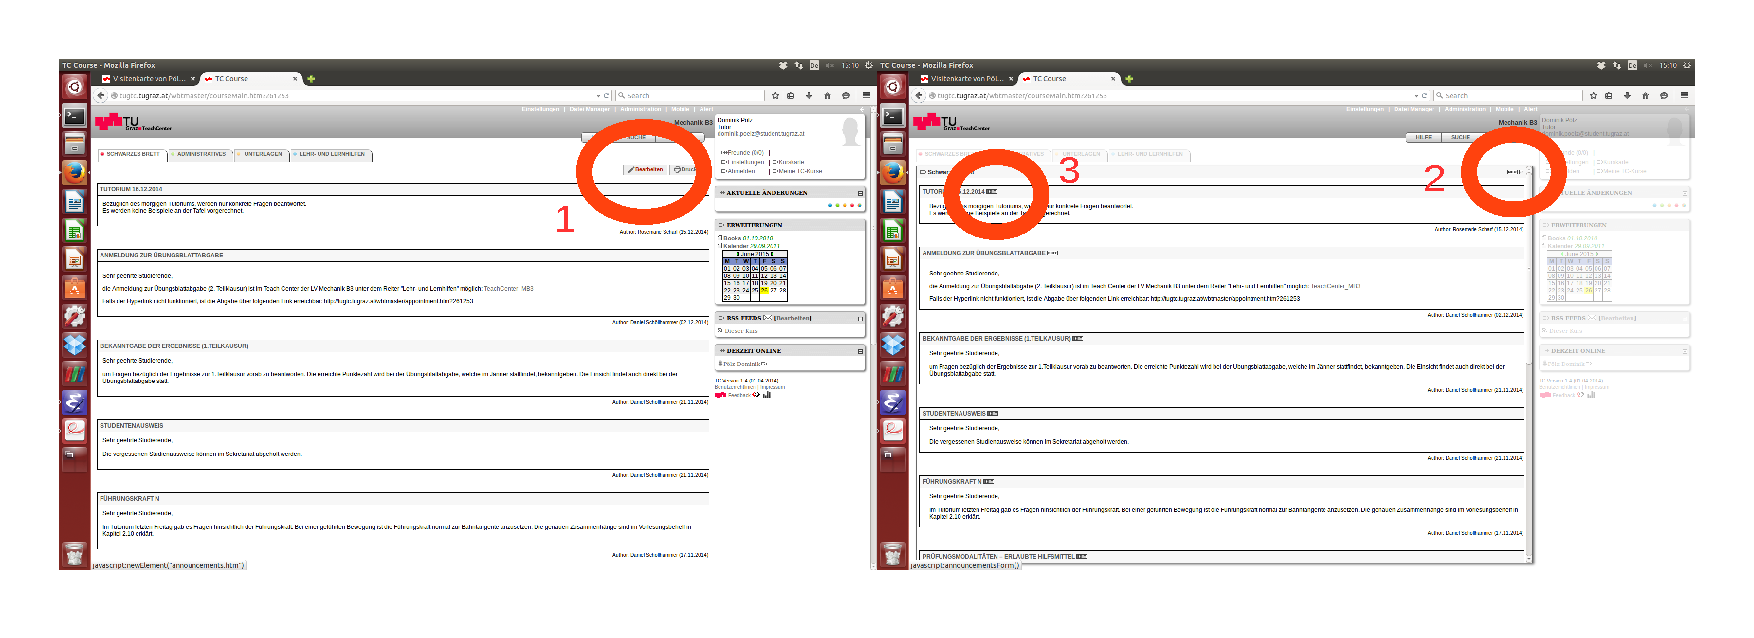
\includegraphics[width=\textwidth]{3_sb.pdf}
  \caption{ (1) Editieren des Schwarzen Brettes. (2) Erstellen eines neuen
    Beitrags. (3) Editieren eines bestehenden Beitrags.}
  \label{fig:sb}
\end{figure}

\section{Administratives}

Hier müssen die {\tt .pdf}-Files des Studenplans und der Prüfungsmodalitäten
hochgeladen werden. Der Prozess ist ähnlich wie beim \twrite{Schwarzen Brett}:
\begin{enumerate}
\item Button \twrite{Bearbeiten}
\item Eingabe von Titel und Text
\item Button \twrite{File hochladen} (unten) um die {\tt .pdf}-Files hochzuladen
\end{enumerate}


\section{Unterlagen}

Hier sind die {\tt .pdf}-Dateien des Vorlesungsbehelfs und der Angabe der
Übungsblätter hochzuladen. Dies funktioniert im Endeffekt gleich wie bei
\twrite{Administratives}:
\begin{enumerate}
\item Button \twrite{Bearbeiten}
\item Links: \twrite{Neues File} $\to$ \twrite{Browse}, Datei auswählen
  $\to$ \twrite{Ok}
\item Rechts: Mit \twrite{Bearbeiten} bestehende files editieren/löschen
\end{enumerate}


\section{Lehr- und Lernhilfen}

Hier müssen einerseits die {\tt .pdf}-Files der durchgerechneten Beispiele und
der Lösungen hochgeladen werden und andererseits die Anmeldung zur 
Übungsblattabgabe erstellt werden. Ersteres funktioniert genau wie bei
\twrite{Unterlagen}.

Grundsätzlich sollte die Gruppeneinteilung vom Vorjahr noch vorhanden sein, und
nicht gelöscht werden. Wurde sie aber gelöscht, so wird eine neue wie folgt
erstellt:
\begin{enumerate}
\item Button \twrite{Bearbeiten}
\item Links: \twrite{Add TC Components} $\to$ \twrite{Kursspezifische Tools}
  $\to$ \twrite{Online-Einteilung}
\end{enumerate}

{\bf Wichtig:}
Wie bereits zu Beginn dieses Kapitels angemerkt, muss diese Anmeldung nur in
der Gruppe {\tt Mechanik B3} erstellt werden, da alle anderen Studierenden
darauf Zugriff haben. Um es einfacher zu gestalten, die Anmeldung
zu finden, sollte in den TC-Gruppen {\tt Dynamik VT} und 
{\tt Mechanik-Dynamik (UE)} ein kurzer Eintrag am Schwarzen Brett erstellt 
werden. In diesem sind die Studierenden darauf zu hinzuweisen, dass die 
Anmeldung zur Übungsblattabgabe in Kürze beginnen wird/gerade begonnen hat und 
diese zu verlinken.

Der Link kann durch einen anchor erstellt werden:\\
\texcode{
<a href= \grqq{}LINK\grqq{}>TeachCenter\_MB3</a>
}

wobei \texcode{LINK} genau jene URL ist, die im Browser angezeigt wird, wenn
man in der Gruppen-Einteilung ist. Zum Vergleich lautete dieser Link
im Studienjahr 2014/15:\\
\texcode{ http://tugtc.tugraz.at/wbtmaster/appointment.htm?261253 }

Die Bezeichnung zwischen \texcode{<a>} und \texcode{</a>} kann natürlich 
beliebig angepasst werden. Weiters ist es sinnvoll, den ganzen Link auch
in textlicher Form im Eintrag am Schwarzen Brett zu inkludieren, zumal
der anchor bei einigen Browser nicht funktionieren könnte.


\subsection{Gruppen-Einteilung (Appointments)}

Die Gruppeneinteilung wird in \figref{fig:groups} dargestellt. Hierbei ist zu
beachten, dass die gesamte Abgabe eines Jahres ein einziges \twrite{Meeting}
ist, und die einzelnen Gruppen TC-intern als \twrite{Groups} bezeichnet werden.
Um sie zu editieren, muss rechts oben auf \twrite{Tools} geklickt werden, und
die einzelnen Aktionen werden im Folgenden noch genauer beschrieben.

\begin{figure}[htbp]
\begin{center}
  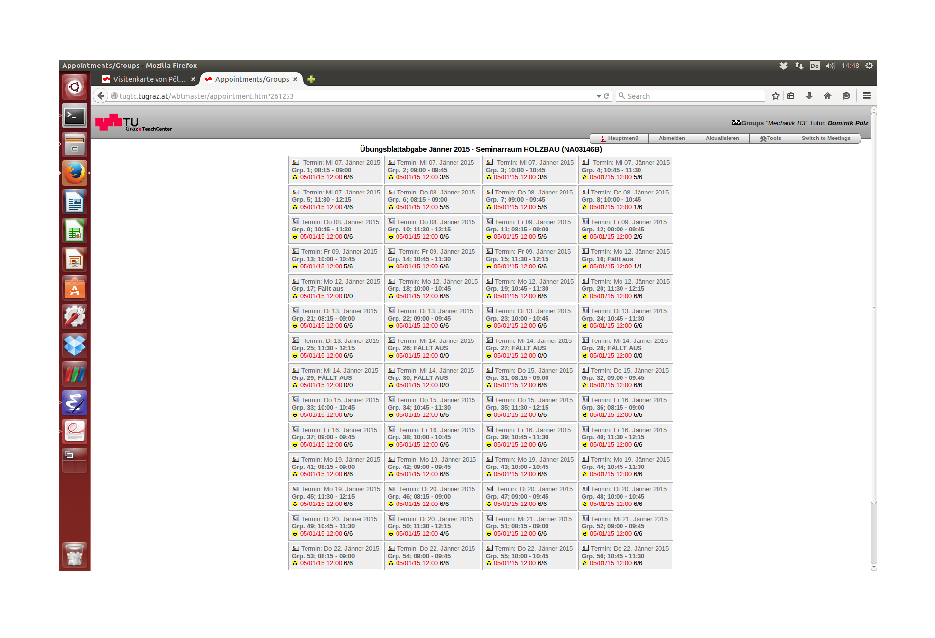
\includegraphics[width=.75\textwidth]{3_groups.pdf}
  \caption{ Gruppen-Einteilung.}
  \label{fig:groups}
\end{center}
\end{figure}

\subsubsection{Tools - Einstellungen}

Unter \twrite{Tools} $\to$ \twrite{Einstellungen} 
(dargestellt in \figref{fig:toolspref}) finden sich die wichtigsten Optionen zur
Übungsblattabgabe:
\begin{itemize}
\item \twrite{Meetings:} Übungsblattabgabe Jänner 20xx\\
  \twrite{Max. Appointments:} 1
\item \twrite{Groups:} Übungsblattabgabe Jänner 20xx - <Raum> (<Raumnummer>)\\
  \twrite{Group Max. Members:} 6
\item \twrite{Sperren/Free:}
  \begin{itemize}
    \item  Anmeldung ab gewissem Zeitpunkt erlauben: 
      \twrite{Sperren till-:} <Zeitpunkt>
    \item  Anmeldung bis zu gewissem Zeitpunkt erlauben: 
      \twrite{Free till-:} <Zeitpunkt>\\
      Muss nicht eingestellt werden, da die Anmeldung bis zu einem gewissen
      Zeitpunkt in den Gruppen erfolgt.
    \item <Zeitpunkt> im Format [yymmddhhmm]: 1501051200 ist beispielsweise
      der 5. Jänner 2015 um 12:00 Uhr.
  \end{itemize}
\end{itemize}

\begin{figure}[htbp]
  \begin{center}
  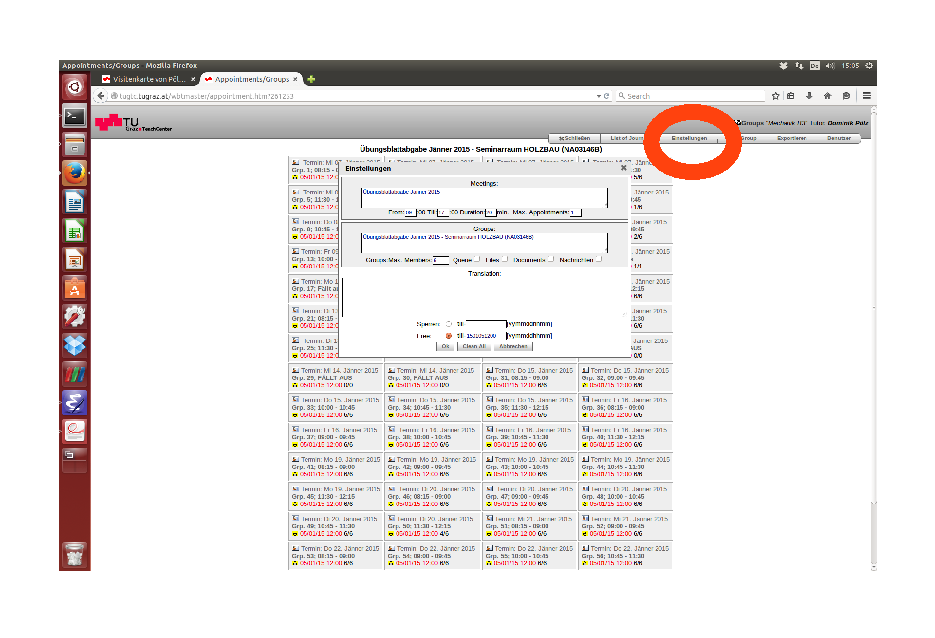
\includegraphics[width=.94\textwidth]{3_toolspref.pdf}
  \caption{ Tools - Einstellungen.}
  \label{fig:toolspref}
  \end{center}
\end{figure}

\subsubsection{Tools - New Group}

Unter \twrite{Tools} $\to$ \twrite{New Group} 
(siehe \figref{fig:toolsnew}) können neue Gruppen erstellt werden:
\begin{itemize}
\item \twrite{Titel:} 
  Hier sollte folgender Vorlagentext hineingeschrieben werden:\\
  \texcode{
    Termin: Mi 07. Jänner 2015<br><strong>Grp. 1; 08:15 - 09:00</strong> }\\
  Die einzelnen Zeiten und Gruppennummern müssen dann noch manuell eingetragen
  werden, aber die richtigen Kommandos für das Layout sind damit schon mal
  aufgesetzt (\twrite{<br>} sorgt für einen Zeilenumbruch und der Text
  zwischen \twrite{<strong>} und \twrite{<\textbackslash strong>} wird fett 
  gedruckt).
\item \twrite{Number of Groups:} xx\\
  So viele Gruppen wie benötigt. Dies ist beispielsweise aus dem Stundenplan 
  ersichtlich.
\item \twrite{Registration till-:}\\
  Hier wird der Endzeitpunkt der Anmeldung für alle Gruppen fixiert, wobei der
  Beginnzeitpunkt bereits in den Einstellungen definiert wurde.  
\end{itemize}

\begin{figure}[htbp]
  \begin{center}
  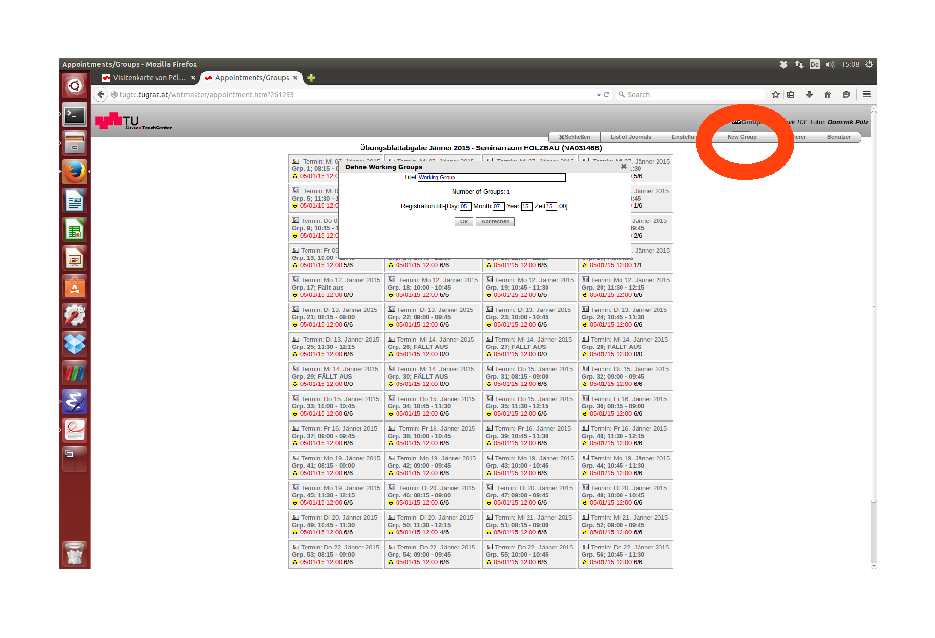
\includegraphics[width=.94\textwidth]{3_toolsnew.pdf}
  \caption{ Tools - New Group.}
  \label{fig:toolsnew}
  \end{center}
\end{figure}

Somit werden alle Gruppen entsprechend der Vorlage erstellt. Nun muss noch jede
Gruppe per Hand mit Nummer und Zeit versehen werde, was im Folgenden beschrieben
wird.

\subsubsection{Gruppe editieren}

Um eine Gruppe zu bearbeiten, klickt man in der Liste aller Gruppen den Titel
der gewünschten Gruppe, der nach der Vorlage 
\glqq{}Termin: Mi 07. Jänner 2015 {\bf Grp. 1; 08:15 - 09:00}\grqq{} lautet.
Darauf öffnet sich ein Fenster, in dem man durch Klick auf \twrite{Bearbeiten}
zu den einzelnen Eigenschaften der Gruppe gelangt (siehe 
\figref{fig:toolsgroup}). Hier muss in jeder Gruppe im Feld \twrite{Titel} das
Datum, die fortlaufende Gruppennummer und die Uhrzeit eingegeben werden.

Sollte ein Termin ausfallen, so kann hier z.B. die Uhrzeit durch 
\glqq{}ENTFÄLLT\grqq{} ersetzt werden und im Feld \twrite{Registration till-}
ein Termin in der Vergangenheit angegeben werden (somit existiert die Gruppe
noch, aber niemand kann sich anmelden).

\begin{figure}[htbp]
  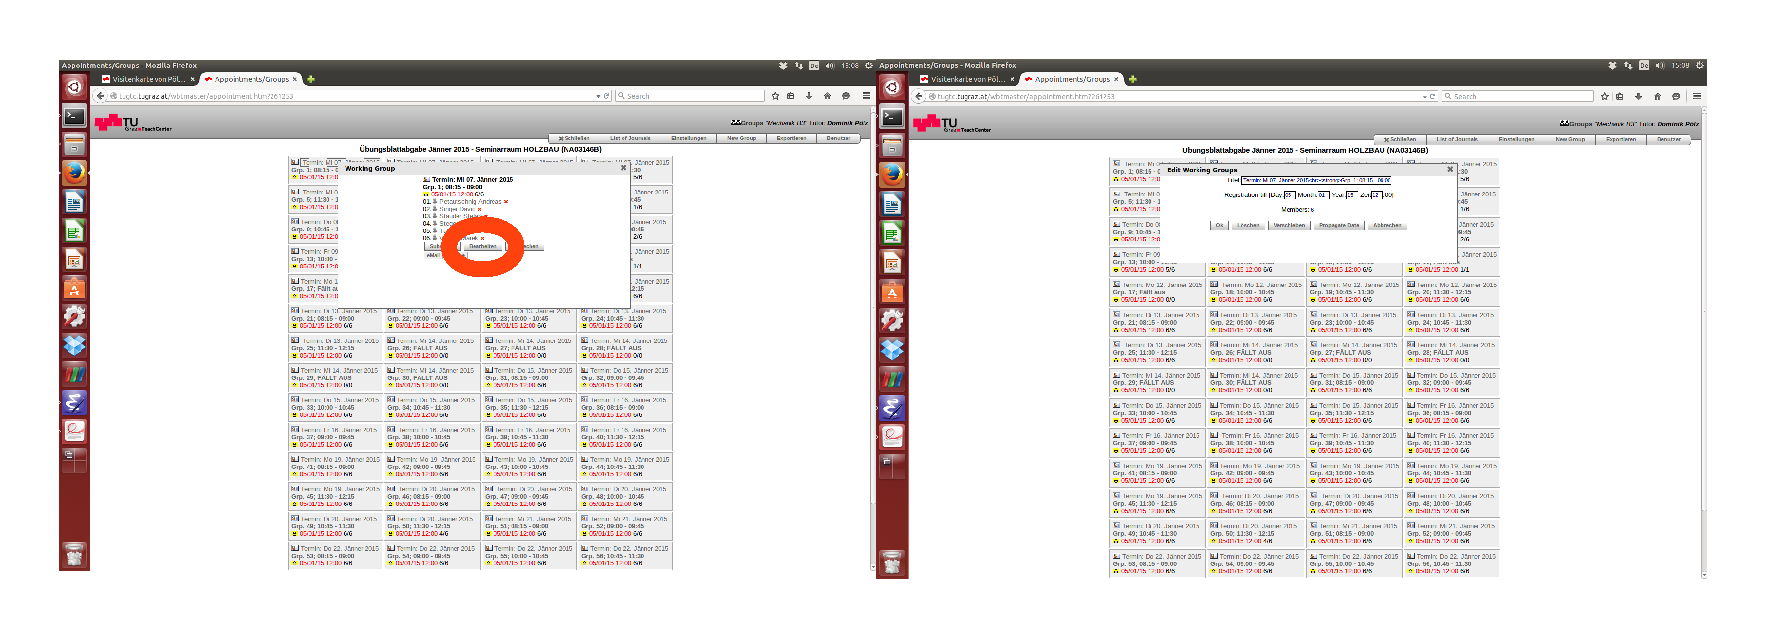
\includegraphics[width=\textwidth]{3_toolsgroup.pdf}
  \caption{ Bearbeiten der einzelnen Gruppen.}
  \label{fig:toolsgroup}
\end{figure}

\newpage
\subsubsection{Exportieren}

Nach Ende der Anmeldefrist muss die Teilnehmerliste jeder Gruppe exportiert
werden. Dieser Prozess wird im Folgenden beschrieben:
\begin{enumerate}
  \item \twrite{Tools} $\to$ \twrite{Exportieren} 
  \item \twrite{All Groups} $\to$ \twrite{CSV} (siehe \figref{fig:exportall})
  \item Im Fenster \twrite{Copy/Paste} {\bf ctrl-a} (alles auswählen) und 
    {\bf ctrl-c} (kopieren) drücken (siehe \figref{fig:copypaste}).
 \item Den Inhalt in einen Texteditor (z.B. \twrite{notepad}, \twrite{notepad++}
    oder \twrite{emacs}) kopieren.
 \item Alle HTML-tags entfernen:
    \begin{itemize}
      \item Ersetze: <br> durch \twrite{void}
      \item Ersetze: <strong> durch \twrite{void}
      \item Ersetze: </strong> durch \twrite{void}
      \item Ersetze: \grqq{} durch \twrite{void} \footnotemark[2]
      \item \twrite{void} bedeutet ein leeres Feld (kein Leerzeichen, sondern
        wirklich Nichts)
    \end{itemize}
  \item Den modifizierten Text mit {\bf ctrl-a} und {\bf ctrl-c} kopieren und
    dann mit {\bf ctrl-v} in Excel einfügen.
  \item Trennsymbol (\glqq{}separator symbol\grqq{}): Hier darf nur das
    Semikolon verwendet werden. Das Leerzeichen (Space) darf nicht verwendet
    werden, da sonst die Aufteilung der Spalten keinen Sinn macht.
\end{enumerate}

\footnotetext[2]{Das Zeichen \grqq{} erhählt man auf deutschen Keyboards durch 
{\bf shift-2}.}

Bei den eigentlichen Excel Dateien der Teilnehmerlisten sollte man sich sehr
stark an den Listen der Vorjahre orientieren, d.h. die Liste des vergangenen
Jahres kopieren und das sheet der {\tt csv} Datei mit der neuen Liste
überschreiben.

\begin{figure}[htbp]
\begin{center}
  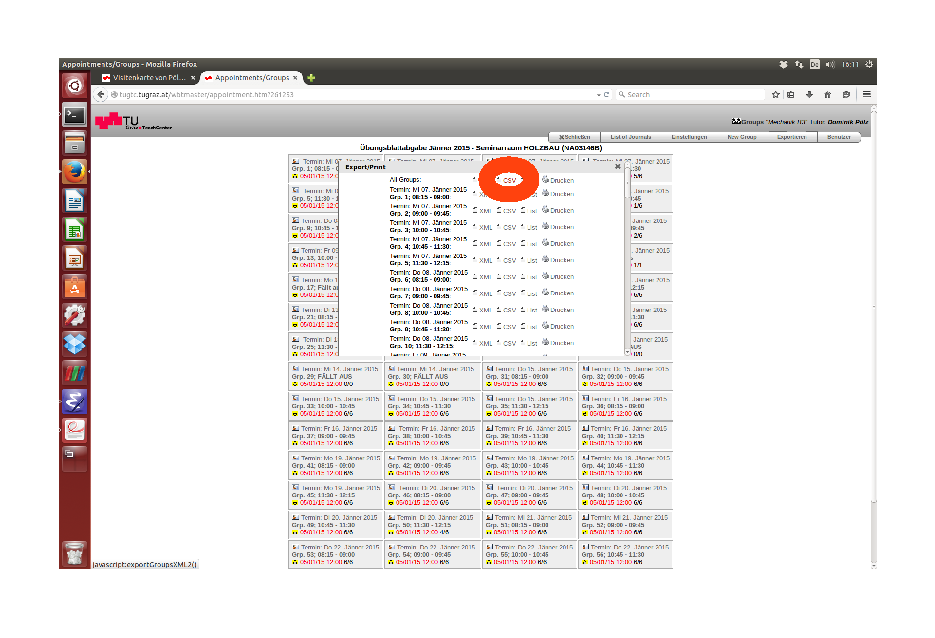
\includegraphics[width=.94\textwidth]{3_exportall.pdf}
  \caption{ Alle Gruppen als {\tt CSV} exportieren.}
  \label{fig:exportall}
\end{center}
\end{figure}

\begin{figure}[htbp]
\begin{center}
  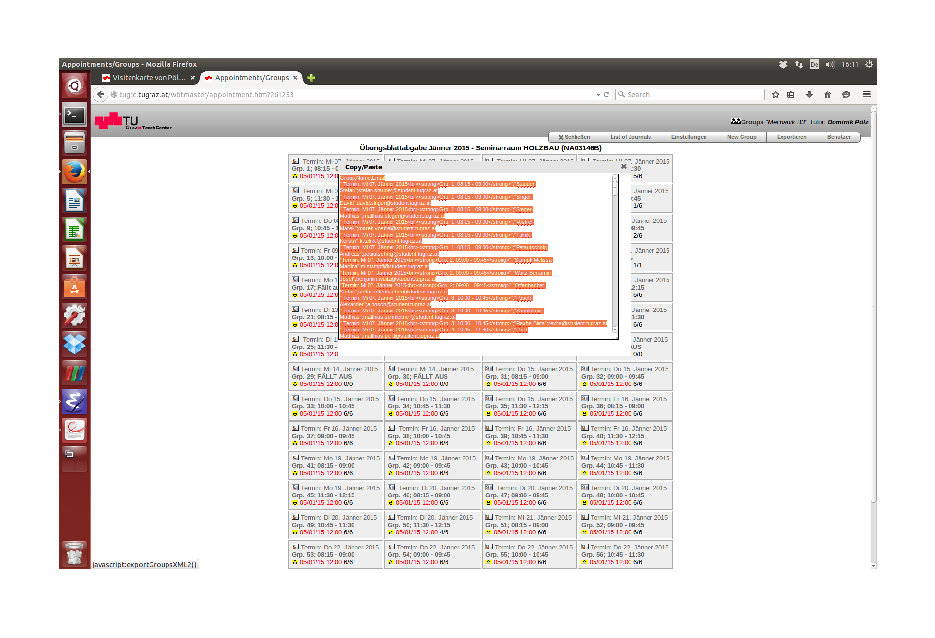
\includegraphics[width=.94\textwidth]{3_copypaste.pdf}
  \caption{ Copy/Paste.}
  \label{fig:copypaste}
\end{center}
\end{figure}

% EOF
%
%% chapter 5 : miscellaneous items
\chapter{Diverses}

% Note: This chapter is intended as some sort of backup. It does not necessarily
% need to hold miscellanea, but anything you deem valuable.

Inhalt.

%EOF
%%%%%%%%%%%%%%%%%%%%%%%%%%%%%%%%%%%%%%%%%%%%%%%%%%%%%%%%%%%%%%%%%%%%%%%%%%%%%%%%

\end{document}
%EOF